%\documentclass[journal]{vgtc}                % final (journal style)
\documentclass[review,journal]{vgtc}         % review (journal style)
%\documentclass[widereview]{vgtc}             % wide-spaced review
%\documentclass[preprint,journal]{vgtc}       % preprint (journal style)

%% Uncomment one of the lines above depending on where your paper is
%% in the conference process. ``review'' and ``widereview'' are for review
%% submission, ``preprint'' is for pre-publication, and the final version
%% doesn't use a specific qualifier.

%% Please use one of the ``review'' options in combination with the
%% assigned online id (see below) ONLY if your paper uses a double blind
%% review process. Some conferences, like IEEE Vis and InfoVis, have NOT
%% in the past.

%% Please use the ``preprint''  option when producing a preprint version
%% for sharing your article on an open access repository

%% Please note that the use of figures other than the optional teaser is not permitted on the first page
%% of the journal version.  Figures should begin on the second page and be
%% in CMYK or Grey scale format, otherwise, colour shifting may occur
%% during the printing process.  Papers submitted with figures other than the optional teaser on the
%% first page will be refused. Also, the teaser figure should only have the
%% width of the abstract as the template enforces it.

%% These few lines make a distinction between latex and pdflatex calls and they
%% bring in essential packages for graphics and font handling.
%% Note that due to the \DeclareGraphicsExtensions{} call it is no longer necessary
%% to provide the the path and extension of a graphics file:
%% 
\includegraphics{diamondrule} is completely sufficient.
%%
\ifpdf%                                % if we use pdflatex
  \pdfoutput=1\relax                   % create PDFs from pdfLaTeX
  \pdfcompresslevel=9                  % PDF Compression
  \pdfoptionpdfminorversion=7          % create PDF 1.7
  \ExecuteOptions{pdftex}
  \usepackage{graphicx}                % allow us to embed graphics files
  \DeclareGraphicsExtensions{.pdf,.png,.jpg,.jpeg} % for pdflatex we expect .pdf, .png, or .jpg files
\else%                                 % else we use pure latex
  \ExecuteOptions{dvips}
  \usepackage{graphicx}                % allow us to embed graphics files
  \DeclareGraphicsExtensions{.eps}     % for pure latex we expect eps files
\fi%

%% it is recomended to use ``\autoref{sec:bla}'' instead of ``Fig.~\ref{sec:bla}''
\graphicspath{{figures/}{pictures/}{images/}{./}} % where to search for the images


\usepackage{pifont}
\usepackage{diagbox}
\usepackage{graphicx}
\usepackage{stfloats}
%\usepackage{algpseudocode}
\usepackage{amsmath,bm}
\usepackage{amsmath}
\usepackage{amssymb}
\usepackage{ragged2e}
\usepackage{algorithm}
\usepackage{algorithmic}
\usepackage{array}
\usepackage{tabularx}
\usepackage{multirow}
\usepackage{makecell}



\usepackage{microtype}                 % use micro-typography (slightly more compact, better to read)
\PassOptionsToPackage{warn}{textcomp}  % to address font issues with \textrightarrow
\usepackage{textcomp}                  % use better special symbols
\usepackage{mathptmx}                  % use matching math font
\usepackage{times}                     % we use Times as the main font
\renewcommand*\ttdefault{txtt}         % a nicer typewriter font
\usepackage{cite}                      % needed to automatically sort the references
\usepackage{tabu}                      % only used for the table example
\usepackage{booktabs}                  % only used for the table example
%% We encourage the use of mathptmx for consistent usage of times font
%% throughout the proceedings. However, if you encounter conflicts
%% with other math-related packages, you may want to disable it.

%% In preprint mode you may define your own headline. If not, the default IEEE copyright message will appear in preprint mode.
%\preprinttext{To appear in IEEE Transactions on Visualization and Computer Graphics.}

%% In preprint mode, this adds a link to the version of the paper on IEEEXplore
%% Uncomment this line when you produce a preprint version of the article
%% after the article receives a DOI for the paper from IEEE
%\ieeedoi{xx.xxxx/TVCG.201x.xxxxxxx}

%% If you are submitting a paper to a conference for review with a double
%% blind reviewing process, please replace the value ``0'' below with your
%% OnlineID. Otherwise, you may safely leave it at ``0''.
\onlineid{1471}

%% declare the category of your paper, only shown in review mode
\vgtccategory{Research}
%% please declare the paper type of your paper to help reviewers, only shown in review mode
%% choices:
%% * algorithm/technique
%% * application/design study
%% * evaluation
%% * system
%% * theory/model
\vgtcpapertype{Representations \& Interaction}

%% Paper title.
\title{$E^2$Storyline: Visualizing the Relationship with\\ Triplet Entities and Event Discovery}

%% This is how authors are specified in the journal style

%% indicate IEEE Member or Student Member in form indicated below
\author{Yunchao Wang, Zihao Zhu, Tong Li, Jiang Qi, Guodao Sun, and Ronghua Liang,\textit{Member,~IEEE}}
\authorfooter{
%% insert punctuation at end of each item
\item
 Yunchao Wang is with Zhejiang University of Technology. E-mail: wyctears@gmail.com.
\item
 Zihao Zhu is with Zhejiang University of Technology, Inc.. E-mail: iszhuzh@outlook.com.
\item
 Tong Li is with Zhejiang University of Technology. E-mail: litong@zjut.edu.cn.
 \item
 Jiang Qi is with Zhejiang University of Technology. E-mail: martha.stewart@marthastewart.com.
 \item
 Guodao Sun is with Zhejiang University of Technology. E-mail: guodao@zjut.edu.cn.
 \item
 Ronghua Liang is with Zhejiang University of Technology. E-mail: rhliang@zjut.edu.cn.
}

%other entries to be set up for journal
\shortauthortitle{Biv \MakeLowercase{\textit{et al.}}: Global Illumination for Fun and Profit}
%\shortauthortitle{Firstauthor \MakeLowercase{\textit{et al.}}: Paper Title}

%% Abstract section. 如何更好的概览故事的发展趋势和实体之间的关系,一直是研究热门。How to get a better overview of story trends and the relationship between entities has always been a popularity of research.
%实体之间的互动,演变成了事件;事件相互串联,组合成了故事。实体之间的动态关系是指故事进程中,实体A与实体B之间的互动。在众多可视化技术中,故事线以其概览故事趋势、揭露实体互动和简化视觉传达方面的有效性和有用性受得到了广泛关注。现有的方法,例如“捆绑”+“阴影”,以隐喻的形式表达某一事件中某些实体存在关联。然而,这种方法不能详细显示实体间的具体关系。在本工作中,我们提出了一种新的故事线可视化形式,在向用户传递更多信息的同时,兼顾简洁美观。我们借助三元组具体展示实体之间的关系。结合用来替代“捆绑”+“阴影”的像素图,增强了信息传达的能力。通过设定新的优化目标,我们将布局优化问题转换为多目标优化,借由Gurobi求解得到简洁的故事线布局。通过用户调查和案例调查,证明该方法可以使用户更好地发现故事中存在的重要事件,理解故事中人物(实体)之间的关系。最后,我们将E^2Storyline分别用于两个真实数据,证明了可以使用户更好地挖掘故事中的信息,了解人物(实体)之间的关系。
\abstract{The relationships between entities form events, which evolve into a story in series. Among the various visualization techniques, storyline visualization has been widely appreciated for its effectiveness and usefulness in providing an overview of story trends, revealing entity relationships, and simplifying visual communication. However, existing storyline visualization methods are	unable to show the specific relationships between entities. In this work, we propose a novel form of storyline visualization, $E^2$Storyline, which takes into account the simplicity and aesthetics of the layout while conveying entity relationship information to users. Firstly, entity relationships are extracted from the text data to form subject-predicate-object(SPO) triples to obtain structured data. After considering the strong design requirements, soft design requirements and custom design requirements, we set new optimization objectives and describe the layout problem as a multi-objective optimization problem. Then the aforementioned SPO triples, time information and event information are fed into the optimization algorithm to ensure a straightforward and easy-to-read storyline layout. Following a qualitative	user study, pixel-based views are proposed to show the relationships between entities. Finally, $E^2$Storyline is applied to two real data individually. It is proven through case studies to let users better uncover the information in the story and understand the relationships between entities.%
} % end of abstract

%% Keywords that describe your work. Will show as 'Index Terms' in journal
%% please capitalize first letter and insert punctuation after last keyword
\keywords{Layout, information visualization, multi-objective optimization, storytelling visualization}

%% ACM Computing Classification System (CCS).
%% See <http://www.acm.org/class/1998/> for details.
%% The ``\CCScat'' command takes four arguments.

\CCScatlist{ % not used in journal version
 \CCScat{K.6.1}{Management of Computing and Information Systems}%
{Project and People Management}{Life Cycle};
 \CCScat{K.7.m}{The Computing Profession}{Miscellaneous}{Ethics}
}

%% A teaser figure can be included as follows
%电影纳尼亚传奇的$E^2$Storyline。参与同一事件的实体在空间上聚集。有交互关系的实体通过带有方向的线段连通。线段头部的不同形状表示不同的行为关系。
\teaser{
  \centering
  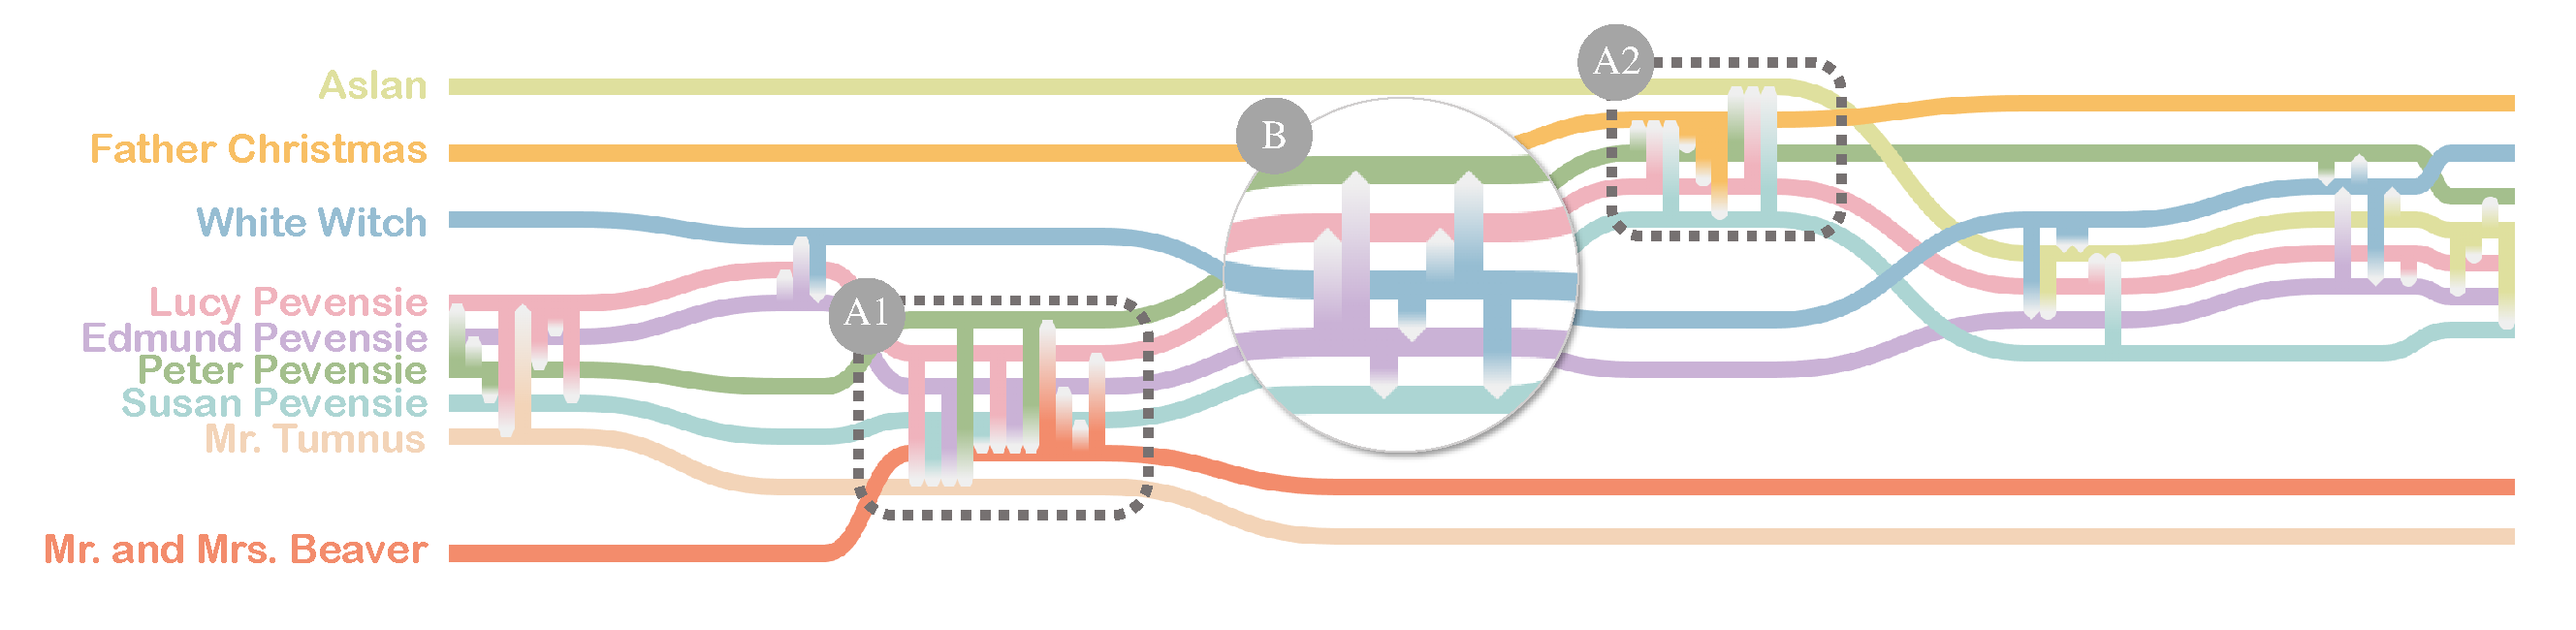
\includegraphics[width=\linewidth]{Fig/firstfig.pdf}
  \caption{$E^2$Storyline for the movie \textit{The Chronicles of Narnia: The Lion, the Witch and the Wardrobe}. Entities participating in the same event are spatially clustered. Entities with interacting relationships are connected by line segments with directions. The different basic shapes of the segment heads indicate different types of relationships.}
  \label{fig:first}
}

%% Uncomment below to disable the manuscript note
%\renewcommand{\manuscriptnotetxt}{}

%% Copyright space is enabled by default as required by guidelines.
%% It is disabled by the 'review' option or via the following command:
% \nocopyrightspace


\vgtcinsertpkg

%%%%%%%%%%%%%%%%%%%%%%%%%%%%%%%%%%%%%%%%%%%%%%%%%%%%%%%%%%%%%%%%
%%%%%%%%%%%%%%%%%%%%%% START OF THE PAPER %%%%%%%%%%%%%%%%%%%%%%The Chronicles of Narnia: The Lion, the Witch and the Wardrobe}. Entities participating in the same event are spatially clustered. Entities with interacting relationships are connected by line segments with directions. The different basic shapes of the segment heads indicate different types of relationships.
%%%%%%%%%%%%%%%%%%%%%%%%%%%%%%%%%%%%%%%%%%%%%%%%%%%%%%%%%%%%%%%%%

\begin{document}

%% The ``\maketitle'' command must be the first command after the
%% ``\begin{document}'' command. It prepares and prints the title block.

%% the only exception to this rule is the \firstsection command
\firstsection{INTRODUCTION}

\maketitle
%在诸如小说、电影、推特话题等数据中,都有由一个或多个事件组成的脉络清晰、层次分明的故事。故事是在时间上或因果关系上相关的一系列事件的总称。
\noindent In data such as novels, movies, Twitter threads, etc., there are well-connected and structured stories consisting of one or more events. Within, for example, novels, movies, Twitter threads, and emails, there are well-paced, layered stories made up of one or more events.
%故事线可视化以其简约性、直观性和有效性,常被用来展示故事发展趋势。其被人们所熟知的形式,在最初Munroe手绘的电影叙事图中就已经有所体现——故事由左往右发展,使用线的形式对实体进行编码,参与同一事件的实体则会聚集在一起。
With its simplicity, immediacy and effectiveness, storyline visualization is often used to show story trends and analyze the relationships between entities. Its familiar form is reflected in the original. 
Munroe~\cite{munroe_movie_nodate} hand-drawn film narrative diagrams. The story develops from left to right, using the form of lines to encode entities, with relationships between entities clustered together.

%我们根据研究重点的不同,将现有故事线可视化相关工作总结为以下3类。第一类工作提出了通用的设计需求和优化目标。这些同样适用在其他领域的时序数据的展示。第二类工作对布局优化算法的性能、算法可靠性等进行分析。第三类对故事线可视化的设计空间做了探讨。但这些工作把注意力放在故事的大致趋势的展现上。尽管通过实体的聚集和分散,用户可以了解每个实体在整个故事中的一些行为模式。但用户无法得知特定情况下,比如某个事件中或某个时刻,实体的具体行为。因此,我们认为,在展示故事大致趋势时,应该兼顾展示实体之间的关系。
According to the different research focuses, we summarize the existing work related to storyline visualization into the following 3 categories. The first category of work presents generic design requirements and optimization goals. These are equally applicable to the presentation of temporal data in other domains. The second category of work analyzes the performance of layout optimization algorithms, algorithm reliability, and other issues. The third category explores the design space for storyline visualization. However, these works focus their attention on the presentation of the general trends of the stories. Although through the aggregation and dispersion of entities, users can understand some behavior patterns of each entity in the overall story.
However, users cannot mine the specific behavior of an entity at the specific time or under the specific event. Therefore, we believe that the presentation of the general trend of the story should be balanced with the presentation of the relationships between the entities.

%实体之间的行为交互构成了事件,不同的事件构成了一个故事流。 
The behavioral interactions between entities constitute events, and the different events constitute a story flow. 
%通过探索实体间的互动,我们可以更好地挖掘实体的行为模式,掌握实体之间的关系。更多地,我们可以借助视觉映射更深刻地理解具体事件、探索事件之间的关联,进一步地了解整个故事。
By exploring the interaction between entities, we can better mine the behavior patterns of entities and grasp the relationship between entities. Moreover, we can better understand specific event and explore the connections between events with the help of visual mapping, and learn more about the overall story.


%关于如何展示故事中各个实体之间动态关系的任务来说,除了要尽可能多的表达信息外,展示方式的简洁直观也是十分重要的。
For the task of showing the dynamic relationships between entities in a story, it is important that the presentation be simple and intuitive, in addition to conveying as much information as possible.
%实体和实体之间的关系,可以用节点链接图来表示。但是节点链接图不适合与故事线可视化结合,因为会产生非常复杂的结构,不易理解与阅读。另一种可视化形式是邻接矩阵。传统的将实体描述为行和列的邻接矩阵,会丢失时间信息。虽然有部分工作将矩阵与时间线结合,但其布局仍旧复杂。
The relationships between entities are often drawn using node-link diagrams. However, the node link graph is not suitable for storyline visualization tasks due to its complex structure. The combination of the two produces a very complex structure that is not easy to understand and read. Another form of graph visualization is the adjacency matrix. The traditional method is to use an adjacency matrix to represent entities, but this method cannot express temporal information intuitively.

%我们提出了一种新的适用于故事线可视化中实体与实体间关系展示的可视化表现。我们将时间描述为矩阵的行,实体描述为矩阵的列。矩阵中某列有颜色的两个单元格表示两个实体之间存在关系。这种设计与故事线可视化的通用形式相契合。
In summary, we propose a visual representation suitable for the display of entity-entity relationships in storylines. We use the rows of the matrix to encode time and the columns of the matrix to encode inter-entity relationships. Two cells in a column of the matrix with color indicate the existence of a relationship between two entities.


%一个简洁的故事线布局是由整体和局部共同作用产生的。整体上我们需要尽可能的减少线的交叉和摆动。局部上我们需要使有关系的实体尽可能的靠近。为此,我们将故事线布局优化描述为多目标优化问题。通过确定目标函数和约束条件对其进行建模,从而确保得到的故事线布局是全局最优的。
A clean storyline layout is produced by a combination of the global and the local. Globally we need to minimize line crossings and wiggles. Locally we need to bring the related entities as close as possible. In conclusion, we describe the storyline layout optimization as a multi-objective optimization problem. It is modeled by determining the objective function and constraints to ensure that the resulting storyline layout is globally optimal.

%具体来说,我们的工作有以下几个贡献。
Specifically, the contributions of our work are as follows.

%一种新的更多细节展示的故事线可视化形式。引入事件和实体与实体间关系,增加了信息表达的数量和质量。
$\bullet$ A novel and more detailed form of storyline. Introducing events and entity-to-entity relationships increases the quantity and quality of information presented.

%一种有效的多目标优化算法,结合多种设计需求,创建简洁直观的故事线布局。
$\bullet$ An effective multi-objective optimization algorithm that combines multiple design requirements to create clean and intuitive storyline layouts.

%多个基于电影简介和文字直播评论的案例评估,证明$E^2$Storyline的可用性和有效性。
$\bullet$ Multiple case evaluations based on movie synopses and live text commentaries demonstrate the usability and effectiveness of $E^2$Storyline.

\section{RELATED WORK}
%     2.1    时间性事件可视化
\subsection{Visualization of temporal events}
%时间性事件可视化是一种基于时间的用来说明事件随时间顺序的可视化技术。由于可视化技术的多样性和广泛可用性,对时间性事件序列数据可视化的总结工作也有不少好的成果。Guo回顾了最先进的视觉分析方法,并提出了新的设计空间对它们进行描述、分类。chao通过对可视化中讲故事的文献进行调查,对其中常见和重要的元素进行概述,并描述了这一领域的挑战。
\noindent Temporal event visualization is a time-based visualization technique used to illustrate events in chronological order. Due to the diversity and widespread availability of visualization techniques, summary work on the visualization of temporal event series data has yielded several favorable results. Guo et al.~\cite{guo_survey_2021} reviewed the state-of-the-art visual analysis methods and proposed a new design space to describe and classify them. Through a survey of the literature on storytelling in visualization, Tong et al.~\cite{tong_storytelling_2018} provided an overview of common and important elements and describes the challenges in this field.

%目前构建时间事件的可视化技术时采用的时间轴的表现形式也有很多。例如:Lifeline,等将时间轴用直线表示。该工作中事件按照其发生的时间在时间线上进行显示。也有一些工作将时间轴用圆形或者弧线表示。StoryPrint,用圆形时间轴的同心圆环对电影中的场景、角色进行可视化表现,并进行比较分析。时间轴形状对任务的性能也存在一定的影响。Sara基于用户任务和数据类型创建有效的时间轴可视化的设计指南。
Many visualization techniques are used to construct temporal events, and the timeline can be represented in many forms. \textit{Lifeline}~\cite{plaisant_lifelines_2003}, for example, represent the timeline as a straight line, in which events are displayed on the timeline according to their time of occurrence. Other work to represent the timeline as a circle or an arc. \textit{StoryPrint}~\cite{watson_storyprint_2019}, a visual representation of scenes and characters in a movie with concentric rings in a circular timeline, and comparative analysis. The shape of the timeline also has an implication on the performance of the task.
Di et al.~\cite{di_bartolomeo_evaluating_2020} create design guidelines for effective timeline visualization based on user tasks and data types.

%通常用于分析事件序列的方法有聚合,细节展示等。常见的聚合形式有桑吉图,冰柱图,以及转移矩阵,它们展示的事件都有相同的时间顺序。尽管它们可以可视化所有事件的排列,但可伸缩性差,不能展示细节层次。通过构建故事概述,或者对事件、时间进行选择或者定义一些规则可以缩减事件规模。用户再借助一些交互手段,可以对细节进行探索分析。为了弥合视觉分析和故事叙述之间的差距,chen提出了一个总体框架,将数据分析和结果展示通过故事合成联系在一起。sequence braiding利用分层有向无环网络对事件时间序列和属性进行总体的可视化。
Typical methods used to analyze event sequences are aggregation, detail presentation, and so on. Some of the common forms of aggregation are Sankey diagrams~\cite{wongsuphasawat_exploring_2012, riehmann_interactive_2005}, icicle diagrams~\cite{monroe_temporal_2013, wongsuphasawat_lifeflow_2011}, and transfer matrices~\cite{yi_timematrix_2010, zhao_matrixwave_2015, bach_visualizing_2014}, which show events in the same chronological order. Although this form of visualization can express the arrangement of all events, it is poorly scalable and cannot show deeper details.
By building an overview of the story~\cite{perer_frequence_2014, liu_coreflow_2017}, or by selection of events and times~\cite{monroe_temporal_2013, baumgartl_search_2020, guo_visual_2018} or by defining some rules~\cite{zgraggen_s_2015, cappers_exploring_2017} can be reduced in size. Users can then explore and analyze the details with the help of interactions~\cite{magallanes_sequen-c_2021, pena-araya_hyperstorylines_2022}. To bridge the gap between visual analysis and storytelling, Chen et al.~\cite{chen_supporting_2018} proposed an overarching framework that links data analysis and presentation of results through story synthesis. \textit{Sequence braiding}~\cite{di_bartolomeo_s_2020} utilized hierarchical directed acyclic networks for the overall visualization of event time series and attributes.

%   2.2   故事线可视化
\subsection{Storyline visualization} 
%故事线可视化作为时间序列可视化中最常用的技术之一,也常常出现在一些工作中。Ogawa在其工作中,提出了一种可视化软件项目演进中开发人员之间交互的技术,可以在展示更多细节的同时,保持对美学和表现的关注。tan提出了一套设计考虑因素,用来产生审美愉悦和易读的故事线可视化。iStoryline通过研究用户如何将叙事转换成手绘故事线,提出了设计空间,并开发了一个创作工具,以求做到手绘故事线和自动布局之间的平衡。PlotThread基于一个强化学习框架来训练人工智能,从而帮助用户探索设计空间,生成优化的故事情节。MeetingVis针对会议数据,提出了一种基于视觉叙事的会议摘要方法。
\noindent Storyline visualization, as one of the most commonly used techniques in time series visualization, also often appeares in some works. Ogawa et al.~\cite{ogawa_software_2010} proposed a technique for visualizing interactions between developers in the evolution of software projects that can show more detail while maintaining a focus on aesthetics and presentation. Tang et al.~\cite{tang_istoryline_2018} proposed a design space \textit{iStoryline} by studying how users convert narratives into hand-drawn storylines.
They also came up with a design space and developed an authoring tool \textit{iStoryline} to strike a balance between hand-drawn storylines and automatic layout.
Tang et al. proposed \textit{PlotThread}~\cite{tang_plotthread_2020} to help users explore the design space and generate optimized storylines.
Based on conference data, Shi et al. proposed a visual narrative-based meeting summary method \textit{MeetingVis}~\cite{shi_meetingvis_2018} for meeting data.

%简洁优美、可读性强的可视化图是该领域研究人员一直追求的。常见的思路是将图中元素按照一定的原则进行位置、大小、形状的改进。也就是对图中的元素布局进行优化。为此,一些设计原则和优化目标被提出,在多个类型的数据中是通用的。在故事线可视化中常见的设计原则有:1、同一集合的(有关系的)的线条应该彼此靠近;2、线条需要保持直到所在的集合(关系)改变。由此提出的设计目标有:1、减少线摆动;2、减少线交叉;3、较少空白区域。Martain将线交叉最小化问题建模成一个带有树约束的多层最小化问题。MetroSet将集合用地铁图的方式进行可视化,并作了布局优化。Martin使用混合整数规划对地铁图布局和标记进行可视化。EvoRiver在减少空白区域做了部分工作。
Clean, elegant and reader-friendly layouts are always pursued by researchers. The common idea is to optimize the element layout, and improve the position, size, and shape of the elements in the diagram according to certain principles. To this end, a number of design principles and optimization goals are proposed that are general across multiple types of data~\cite{tanahashi_design_2012, liu_storyflow_2013, tanahashi_efficient_2015}. The design principles in storyline visualization are: Lines from the same set (with relationships) should be close to each other; Lines need to be maintained until the set (relationship) in which they are located changes. The resulting design goals are: less line wiggling; less line crossings; and less white space. Martain et al.~\cite{gronemann_crossing_2016} modeled the line crossing minimization problem as a multilayer minimization problem with tree constraints. \textit{MetroSet}~\cite{jacobsen_metrosets_2020} visualized sets in terms of Metro maps with layout optimization. Martin et al.~\cite{nollenburg_drawing_2010} used mixed integer programming to visualize the Metro map layout and labeling. \textit{EvoRiver}~\cite{sun_evoriver_2014} focuses on the state-transition optimization for river-based visualization.

%隐喻是有效性和美观性结合的产物,可以在兼顾美观的同时,传达更多的信息。在故事线可视化中,用不同的颜色绘制背景区域可以表达层次信息。SplitStreams用了新颖的视觉隐喻,提供了随时间变化的层次结构的静态概述。除此之外,视觉隐喻的形式也可以采用著名的艺术作品。
Metaphors are the product of combining validity and aesthetics, which can convey more information while taking into account esthetics.  \textit{SplitStreams}~\cite{bolte_splitstreams_2020} used a novel visual metaphor to provide a static overview of the hierarchy over time. Beyond that, visual metaphors can also take the form of prominent artworks~\cite{zhang_visual_2022}.

%上述工作不能在反映故事趋势的同时兼顾实体间关系的展示。我们从整体和部分两个角度对故事线布局优化进行了探索。为此,我们把故事线布局优化描述成多目标优化问题。通过对多目标优化进行求解,从而得到满足优化目标的布局。
The above work cannot reflect story trends while taking into account the presentation of relationships between entities. We explore storyline layout optimization from both global and local perspectives. To this end, we describe the storyline layout optimization as a multi-objective optimization problem, which is solved to obtain a layout that satisfies the optimization objective.

% overview 图
%$E^2$Storylinepipeline。选择具有强时间特性的本文数据作为本文的工作基础。数据处理阶段包含SPO三元组、时间线和事件的提取。优化阶段遵循三种设计需求,提出优化目标和相应的限制条件,进一步实现优化求解。视觉设计阶段包含一个基于实体关系的的故事线布局。
\begin{figure*}[h]
	\centering
	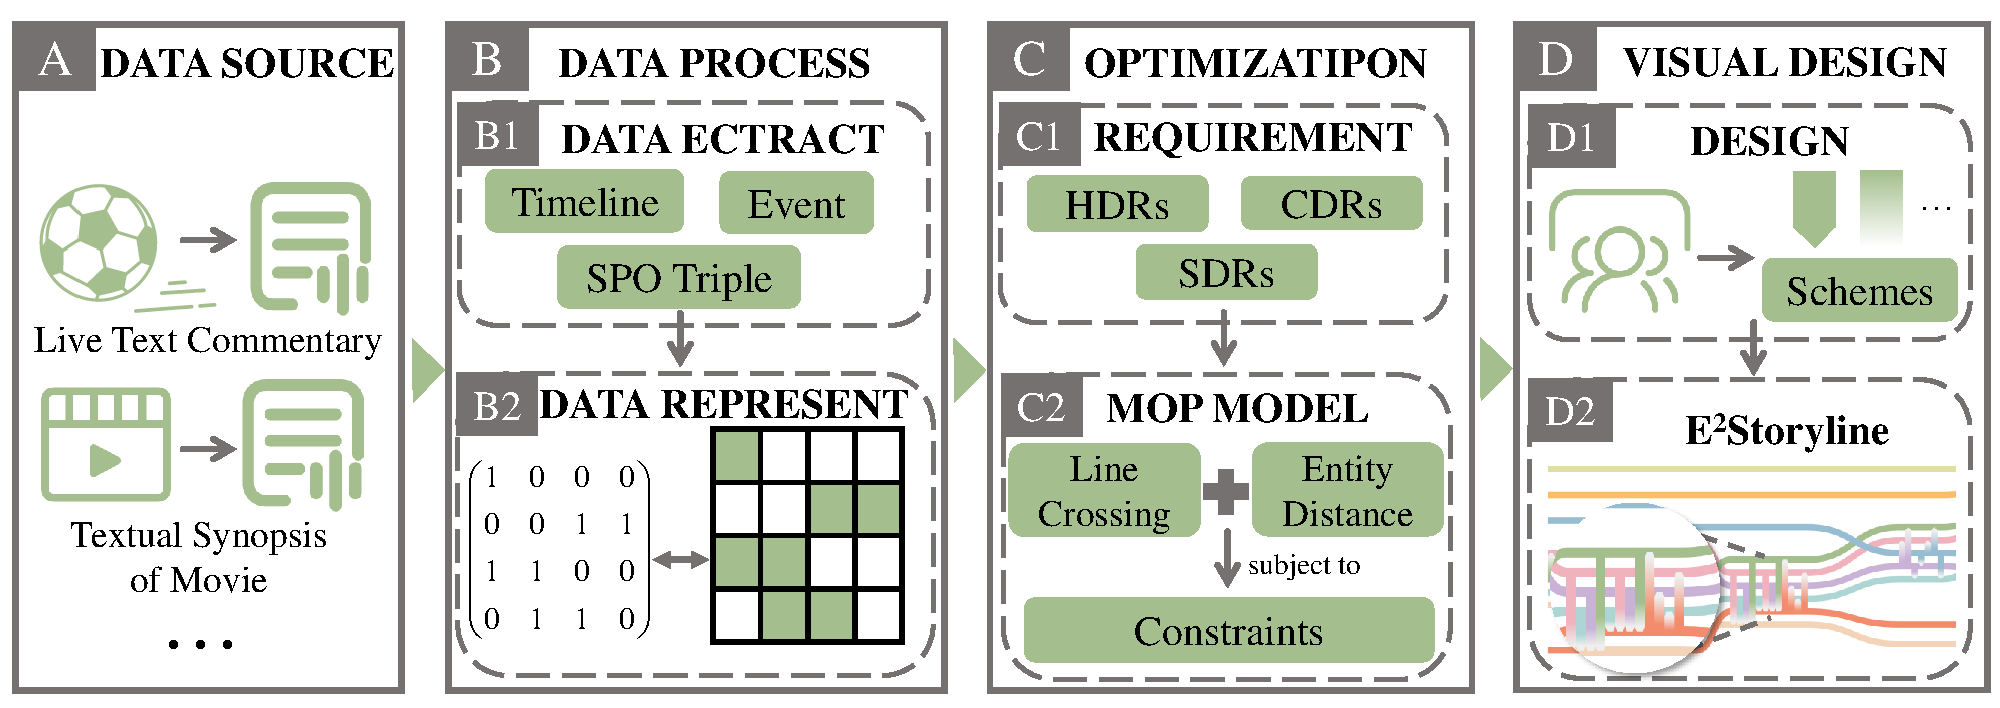
\includegraphics[width=\textwidth]{Fig/overview.pdf}
	\vspace{-1em}
	\caption{The pipeline of $E^2$Storyline. Text data with strong temporal characteristics is selected as the basis of this paper. Data process stage includes the extraction of SPO triples, timeline, and event. The optimization stage follows three design requirements, proposes optimization objectives and corresponding constraints, and further realizes the optimal solution. The visual design stage includes a storyline layout based on entity relationships.}
	\vspace{-1em}
	\label{fig:overview}
\end{figure*}


%    3    %     本节的主要内容是讲述一些思考的点和考虑
\section{CONSIDERATIONS}
%在故事线可视化中加入文本中的事件,以及参与事件的各个实体之间的关系,可以更直观的展示蕴涵的信息、更好的解释实体之间的关系和各个实体的功能。为此,我们提出了E^2Storyline,其目标是生成清晰、可读性高,并能展示实体间具体关系的故事线可视化。在本节中,我们将就数据及可视化设计时考虑的因素进行说明。
\noindent Incorporating events into storyline visualization, and the relationships between various entities in the event, allows for a more intuitive presentation of the information contained in the story, better explanation of the relationships between entities and the roles of each entity. For this purpose, we propose $E^2$Storyline, whose goal is to generate storyline visualizations that are legible, intelligible, and demonstrate the actual relationship among entities. In this section, the considerations for input data and visualization design are illustrated.

%	3.1   数据要求
\subsection{Data Acquisition Requirements}
%故事可以用图书、杂志、电影、博客、论坛、电子邮件等多种媒介上呈现或发行。如图2中所示,数据源可以是实时文字评论,也可以是电影的文字简介。我们所使用的数据源是基于文字的强线性时间线的。选择这类数据源的理由如下:
\noindent Stories can be presented or distributed in a variety of media such as books, magazines, movies, blogs, forums, emails, etc. As shown in Fig~\ref{fig:overview}, the data source can be either live text commentaries or textual synopsis of movies. The data sources we use are text-based with a strong linear timeline. The reasons for choosing this type of data source are as follows.

%线性时间线。故事发展是有时间脉络的。时间在故事发展中是不可或缺的维度之一。为了让故事更加具有吸引力,在小说、电影等艺术性较强的文学作品中,时间会有交错的情况。但在社交媒体、网络文字直播等新兴媒体中,时间通常是线性的。一个具有良好线性时间的文本内容可以更好的用故事线可视化进行展示。
$\blacktriangle$ \textbf{Linear timeline.} Story development is temporal in nature. The timeline is an essential dimension in the development of stories. In literary works with strong artistic quality such as novels and movies, in order to make the story more attractive, there will be plots interlaced in time and space. To make the story more attractive, time is staggered in strong artistic literature such as novels and movies. However, in emerging media such as social media and online text broadcasts, time is usually linear. A textual content with good linear time can be better presented with storyline visualization.  

%便捷的事件提取。近些年随着人工智能的发展,从例如电影,电视剧,电台等基于音频和视频的数据源中也可以进行事件的区分和提取。但是使用基于文字的数据源代价更小,且得到的结果相近。
$\blacktriangle$ \textbf{Convenient event extraction.} In recent years, with the development of artificial intelligence, it is possible to differentiate and extract events from audio and video-based data sources such as movies, TV shows, and radio stations. However, using text-based data sources is cost effective and yields similar results.

%数据编码。基于文本的故事中对两个实体之间关系通常需要用长句进行描述。这种表达方式不够简练。我们需要寻找新的编码方式。新的方式需要具备以下性质:1.结构化。它具有结构化的形式。结构化的形式可以减少文本的存储空间,使数据更易处理。2.记录实体。它能记录参与的实体。记录的实体可以在后续模式探索时发挥作用。3.表达关系。它能表达实体之间的关系。保留实体间的关系可以减少信息丢失,更易发现实体的行为模式。%在自然语言处理中,结构为<Subject-Predicate-Object>(SPO)的三元组可以用来编码带有语义数据的句子。SPO三元组中包含了行为属性的施者和受者。尽管是离散抽取SPO三元组的,但其仍具有时间信息,且对整体趋势不会产生干扰。鉴于此,我们可以按照故事中出现的先后顺序,对角色和行为进行SPO三元组抽取。
$\blacktriangle$ \textbf{Relation encoding.} The relationship between two entities in a text-based story usually needs to be described in long sentences. Such expressions are not concise enough. Therefore, we need to find an efficient way to encode the data. The new approach needs to have the following properties: \ding{182} \textbf{Structured form}. It has a structured form. The structured form reduces the storage space for text and makes the data easier to handle. \ding{183} \textbf{Recorded entity}. It can record the entities involved. The recorded entities can be useful in subsequent model exploration. \ding{184} \textbf{Express relationships}. It can express the relationships between entities. Preserving the relationships between entities reduces information loss and makes it easier to discover the behavior patterns of entities. In natural language processing, a triple with the structure \textit{$<$Subject-Predicate-Object$>$} \textbf{(SPO)}~\cite{hoffart_yago2_2013} can be used to encode sentences with semantic data. An SPO triple contains both the giver (\textit{subject}) and the receiver (\textit{object}) of the action (\textit{predicate}). In view of this, we extract SPO triples for characters and actions in the order of their appearance in the story. While the SPO triples are extracted discretely, they still have temporal information and the overall trend is not disturbed. In view of this, we extract SPO triads for characters and behaviors in the order of their appearance in the story.

%我们使用了两个真实数据。一个是欧冠2015-2016赛季16强,巴塞罗那对阵阿森纳第一回合的文字直播数据。该数据具有很强的线性时间性。我们结合赛后集锦寻找比赛中的事件。另一个是电影《纳尼亚传奇》,我们根据维基百科中的电影简介以及电影本身标注事件。
We used two types of text data that satisfy the above requirements. One type is live text commentary. We selected the live text commentary of \textit{the Champions League} 2015-2016 Round of 16, Barcelona vs. Arsenal first leg. This data is highly linear in time. We combine it with post-match video highlights to find the events in the match. Another type is movie text synopses, we selected \textit{The Chronicles of Narnia: The Lion, the Witch and the Wardrobe}, \textit{Rumble in the Bronx} and \textit{The Matrix}, and we labeled events based on the movie synopses on Wikipedia as well as the movies themselves.


%	3.2   设计需求
\subsection{Design Requirements}
% 设计需求在各类可视化展现中是普遍存在的,也是至关重要的。针对故事线可视化,根据需求的通用性程度,我们提出了三种不同层级的设计需求,分别是硬设计需求,软设计需求和自定义设计需求。
\noindent Design requirements are ubiquitous and crucial in various visual presentations~\cite{tanahashi_design_2012}. For the storyline visualization, we proposed three different levels of design requirements based on the degree of generality of the requirements: Hard Design Requirements, Soft Design Requirements, and Custom Design Requirements.

%HDR的示意图。
%硬设计要求示意图(\textbf{HDR}s)。 (a) 实体用线条编码,时间方向从左到右。 (b) 实体间的聚合和分散内涵了故事的演变。
\begin{figure}[h]
	\centering
	\vspace{0em}	
	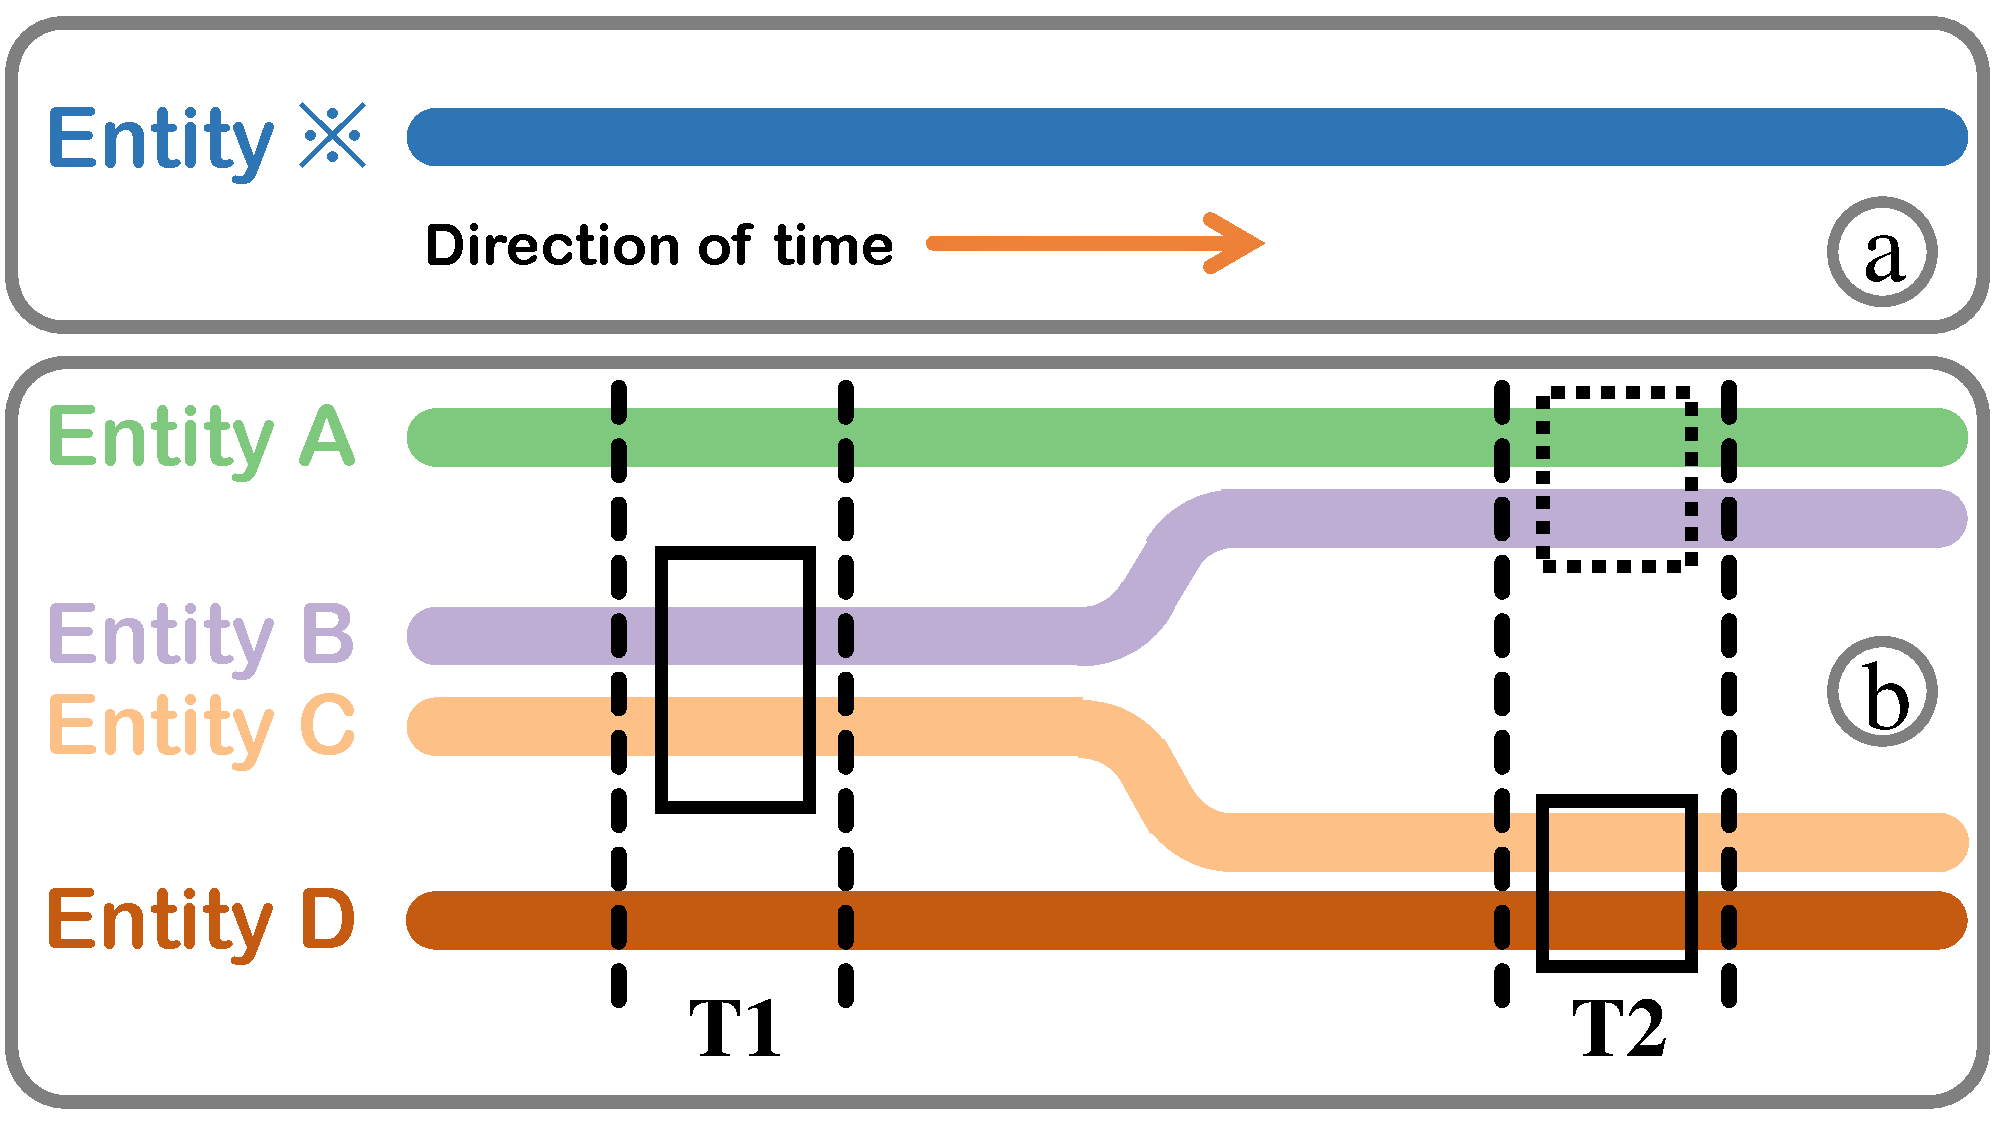
\includegraphics[width=0.38\textwidth]{Fig/HDR.pdf}
	\vspace{-0.5em}
	\caption{Schematic diagram of Hard Design Requirements (\textbf{HDR}s). (a) Entities are encoded with lines and time flows from left to right. (b) The aggregation and dispersion of entities connotes the evolution of the story.}
	\vspace{-0.5em}
	\label{fig:HDR}
\end{figure}

%	3.2.1	硬需求Munroe~\cite{munroe_movie_nodate} hand-drawn film narrative diagrams
\subsubsection{Hard Design Requirements}
%故事线可视化有两个设计要求是共识的。它们分别是“用线编码实体”和“实体聚合和分散”。它们可以追溯到Munroe的手绘电影叙述图。我们将它们定义为硬性设计要求。它们是故事线可视化默认遵守的设计要求。
\noindent Two design requirements for storyline visualization are consensual: ``encoding entities with the lines" and ``aggregation and dispersion of entities", which can be traced back to Munroe's~\cite{munroe_movie_nodate} hand-drawn movie narrative diagrams. We define them as Hard Design Requirements (\textbf{HDR}s). They are considered as the default design requirements for storyline visualization.

%HDR1:用一条随时间发展从左至右延展的线表示实体。线的起始和结尾,表示实体出现和消失的时间点。线的长度表示实体在故事中的寿命。
\ding{118}  \textbf{HDR1: Using a line that extends from left to right as time progresses to represent the entity.} The start and end of the line, indicating the points in time when the entity appears and disappears. The length of the line represents the lifespan of the entity in the story.

%HDR2:用线条的聚集和发散表示实体是否参与同一个事件。如果某段时间某些实体参与了同一个事件,代表这些实体的线就会聚在一起。反之则会发散,或者不会有明显的聚集过程。
\ding{118}  \textbf{HDR2: Using the aggregation and divergence of lines to indicate whether entities participate in the same event.} If certain entities participate in the same event at a certain time, the lines representing those entities will come together. Otherwise, it will diverge, or there will be no obvious aggregation process.



%如图HDR.a:解释HDR1,蓝色的线表示Entity ※, 橙色箭头表示时间。图HDR.b:解释了HDR2,实体A、B、C和D分别用绿色、紫色、橙色和红色表示。在T1时刻,实体B和C有关系,因此它们聚集在一起;在T2时刻,实体A和B有关系,实体C和D有关系,而实体B和C没有关系,因此实体B和C分开,分别与实体A和D聚集。
As shown in Fig~\ref{fig:HDR}.(a), the time progression of the storyline is drawn from left to right. The story flow of the entity is laid out in this direction. 
As shown in Fig~\ref{fig:HDR}.(b), the 4 entities are encoded with four colors respectively. At time T1, entity B and C are related, therefore they are clustered together. 
At time T2, in addition to entity B and C, there is an interaction between entity A and B, an interaction between entity C and D. 
Thus the first group is spatially separated and the latter two groups are spatially clustered.

%	3.2.2	软需求
\subsubsection{Soft Design Requirements}
%故事线可视化作为一种向用户传递信息的表达方式,简洁直观是十分重要。为了达到这个目标,研究人员在遵守硬性设计要求的基础上,还需要解决视觉干扰问题。由于实体采用线条进行编码,在故事线可视化中,视觉干扰较大的主要是线交叉和线摆动。软性设计需求的提出就是要降低这两者带来的视觉干扰。软性设计要求是指,设计要求相同,但实现的方式可以不同。storyflow中为了减少线交叉和线摆动,采用了两阶段的方法:首先生成一组关系树,然后进行行排序和行对齐。类似的在“sequence braiding”中,采用了“rank assignment”, “building the graph”,“within-rank node sorting” 和 “linear programming for exact intersection reduction”等步骤来减少线交叉和线摆动。总的来说,针对线摆动和线交叉的软性设计要求具体内容如下:
\noindent As a way of conveying information to users, storyline visualization is important to be concise and intuitive. To achieve this goal, researchers need to address visual interference in addition to complying with hard design requirements. Since entities are encoded using lines, the main visual disturbances in storyline visualization are line crossings and line wiggles. The soft design requirements are proposed to alleviate the above problems. Soft design requirements mean that the design requirements are the same, but the implementation can be different. A two-stage approach is used in \textit{StoryFlow}~\cite{liu_storyflow_2013} to reduce line crossing and line wiggling: first a set of relationship trees is generated, then line sorting and line alignment is performed. Similarly, in \textit{Sequence Braiding}~\cite{di_bartolomeo_s_2020}, ``rank assignment", ``building the graph", ``within-rank node sorting" and ``linear programming for exact intersection reduction" are used to reduce line crossings and line wiggles. Generally speaking, the soft design requirements for line wiggles and line crossings are specified as follows: 

%SDR1:减少线交叉个数。较少的线交叉可以降低视图的复杂程度,减少用户阅读负担,更好的理解视图中蕴含的信息。
\ding{117}  \textbf{SDR1: Reduce the number of line crossings.} Fewer line crossings can reduce the complexity of the view, reduce the user's reading burden, and better understand the information contained in the view.

%SDR2:减少线摆动次数。过多的或者没必要的线摆动,不仅在视觉上会产生线条的不连续性,同时还会变相增加线交叉个数。
\ding{117}  \textbf{SDR2: Reduce the number of line swings.} Excessive or unnecessary line swings will not only visually produce line discontinuities, but also increase the number of line crossings in disguised form.


%	3.2.3	自定义需求
\subsubsection{Custom Design Requirements}
%由于故事线可视化应用的领域的多样性,数据和视觉表达的侧重点也会有所不同。“Sequence Braiding”针对1型糖尿病治疗案例,收集了设计要求,并以此作为设计、实现和布局算法的依据。为了在故事线可视化中显示事件中实体之间的关系,除了我们坚持的硬性和软性设计要求外,我们还增加了两个自定义设计要求。
\noindent Due to the diversity of areas where storyline visualization is applied, the focus of the data and visual representation varies. In \textit{Sequence Braiding}~\cite{di_bartolomeo_s_2020}, design requirements are collected for the design, implementation and layout of the algorithm for the type 1 diabetes treatment case. In order to show the relationship between entities in an event in the storyline visualization, we have added two Custom Design Requirements (\textbf{CDR}s) in addition to the HDRs and SDRs.

%CDR1:用矩阵$M_(i,j)$描述事件。矩阵的行代表实体,行的索引为实体在矩阵中的位置,列代表三元组,列的索引为SPO三元组发生的顺序。举个例子,如图4中橙色框内表示事件中的第三条SPO三元组。在第三个SPO三元组中($j=3$)实体A($i_A=1$)和实体C($i_C=3$)有关系,则$M_{(1,1)} = 1$, $M_{(3,1)} = 1$.为了形象地表达该事件矩阵,我们引入了像素图。为了方便区分,我们用不同的颜色进行了区分,如图5,
\ding{108}  \textbf{CDR1: Represent the entities involved in the same event in an intuitive way.} We use the matrix \textbf{$M_{x,y}$} to describe events. The rows of the matrix represent entities, and the index of the rows  ($y$) is the position of the entities in the matrix. The columns represent the triples, and the index of the columns ($x$) is the order in which the SPO triples occur. The left side of Fig~\ref{fig:m2p} shows the events described with the matrix $M$.  As an example, the orange box in Fig~\ref{fig:m2p} represents the third SPO triple in the event. In the third SPO triple ($x = 3$), entity B ($y_B = 4$) and entity D ($y_D = 2$) have a relationship, then $M_{3,2} = 1$ and $M_{3,4} = 1$. To vividly represent this event matrix, we introduce the pixel map. The right side of Fig~\ref{fig:m2p} shows the pixel map instead of the matrix. The value of ``1" in the matrix is filled with color in the pixel map, while the value of ``0" is not used. To facilitate the distinction, we have distinguished them with different colors, as shown in Fig~\ref{fig:CDR}.

% 矩阵转像素图
%\textbf{CDR}1 的示意图。左侧矩阵描述一个事件。矩阵的行代表不同的实体, 矩阵的列代表SPO 三元组。进一步用右侧像素图来映射事件矩阵。 橙色框标识实体 B 和 D 的 SPO 三元组关系。
\begin{figure}[h]
	\centering
	\vspace{-0.5em}
	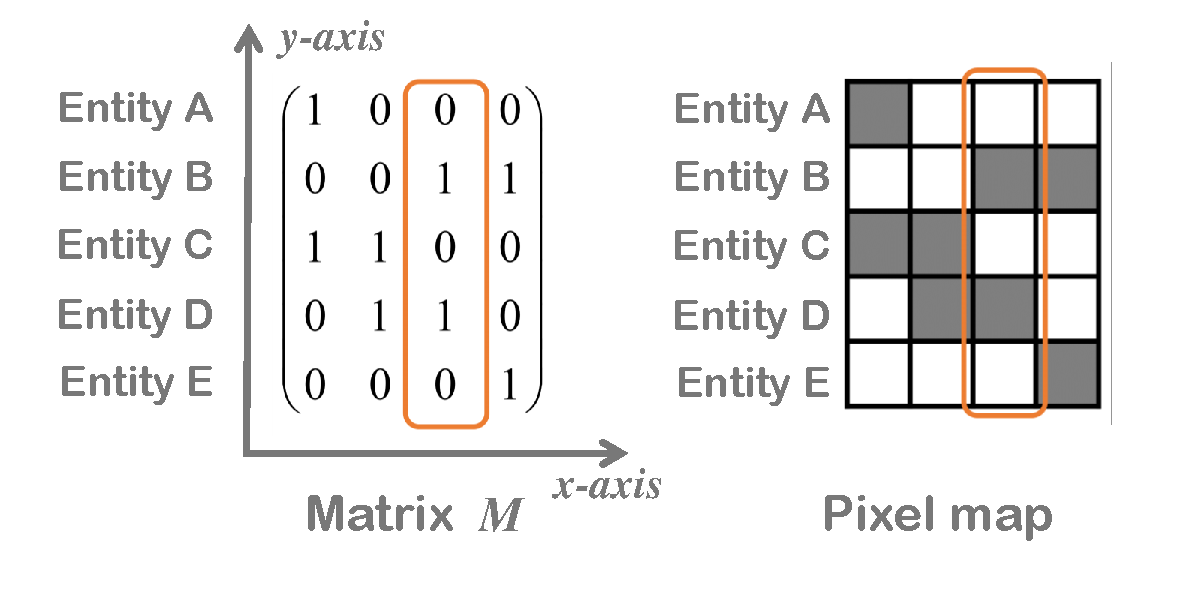
\includegraphics[width=0.46\textwidth]{Fig/matrix2pixelmap.pdf}
	\vspace{-1em}
	\caption{Schematic diagram of Custom Design Requirements 1 (\textbf{CDR}1). The matrix on the left describes an event. The rows of the matrix represent different entities, and the columns represent SPO triples. Further map the event matrix with the pixel map on the right. The highlighted box identifies the SPO triple relationship for entity B and D.}
	\vspace{-1.5em}
	\label{fig:m2p}
\end{figure}

%CDR的示意图。
%\textbf{CDR}2的示意图。 (a) 像素图用于描述事件$\star$。 x 轴表示SPO 三元组的时间顺序,y 轴表示实体顺序。 (b) 考虑实体之间的关系,进一步优化实体位置,彼此靠近。
\begin{figure}[h]
	\centering
	\vspace{-0.5em}
	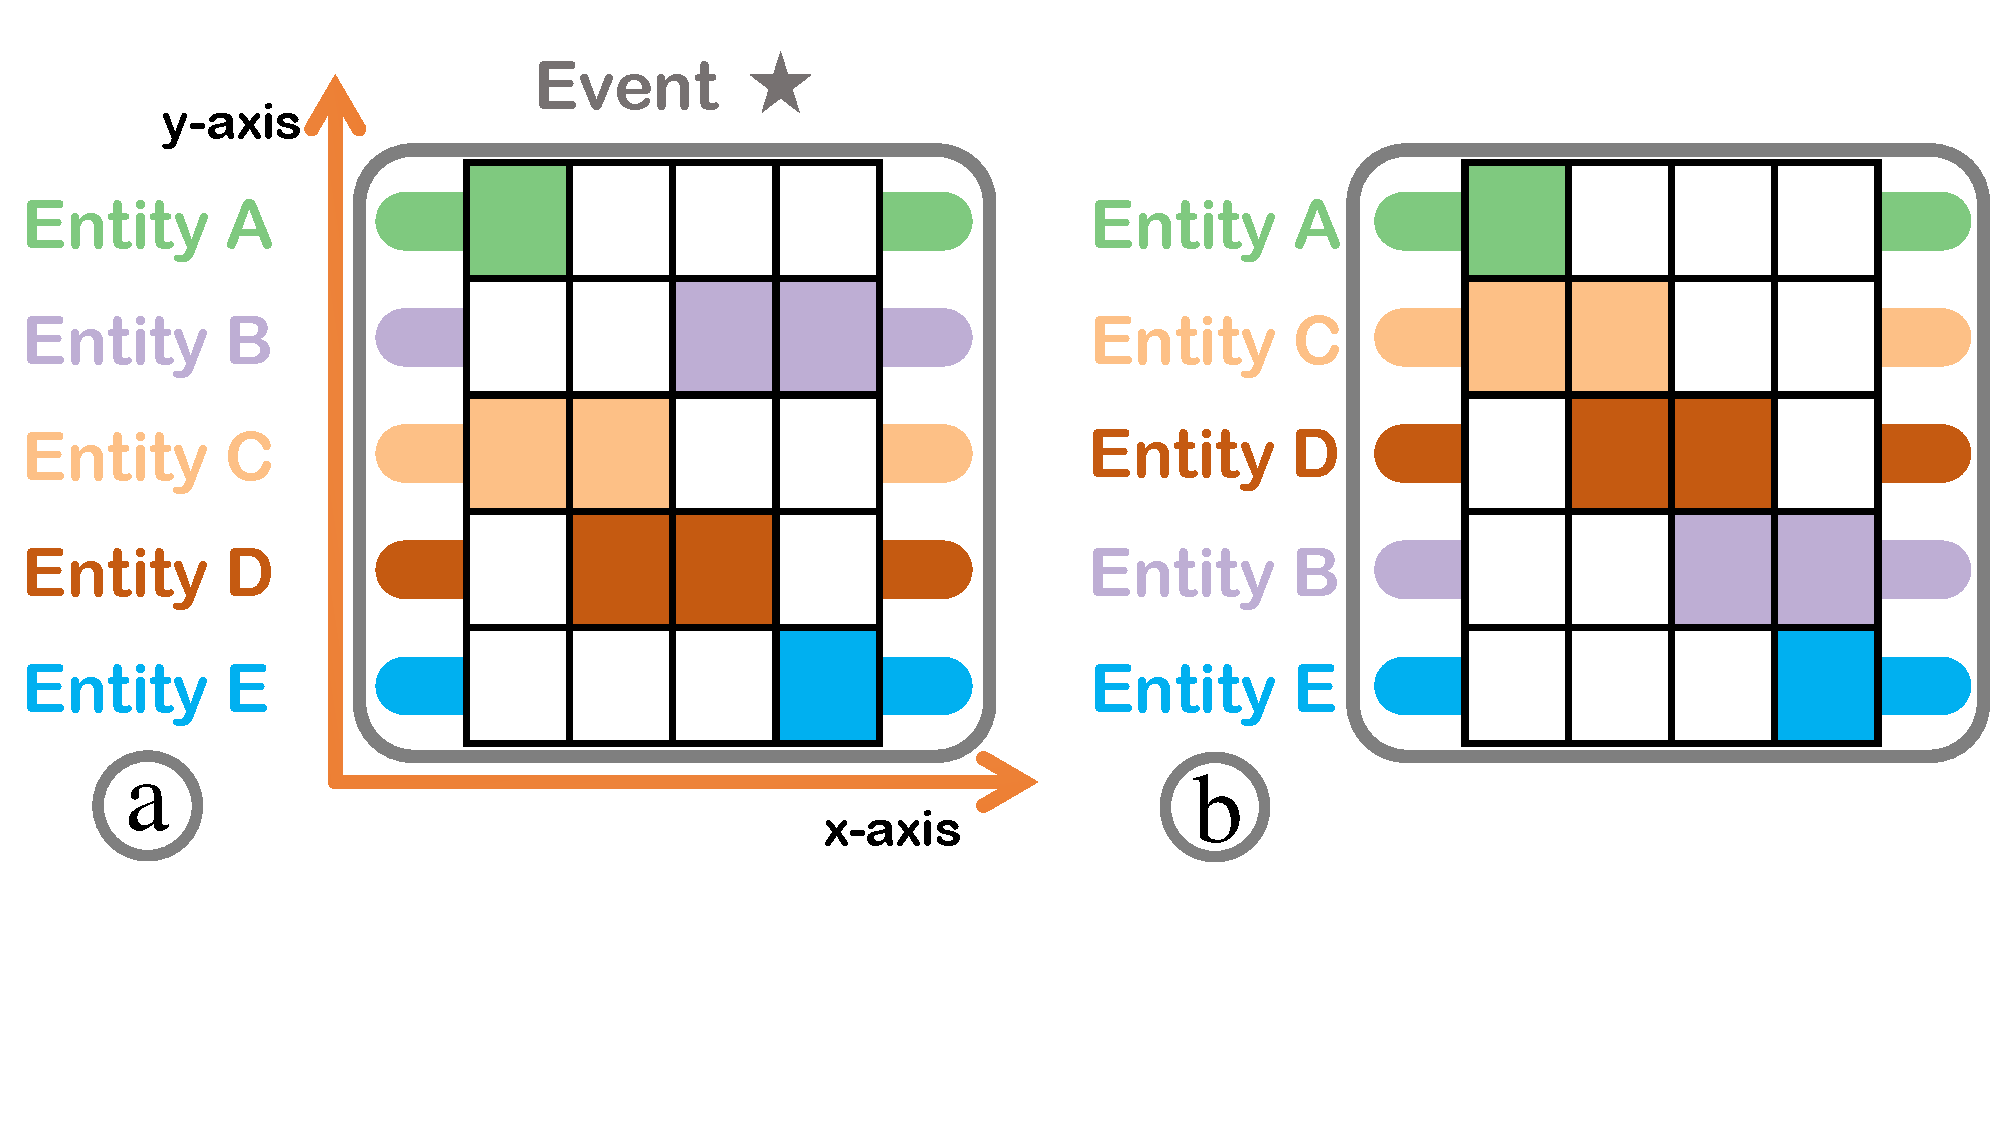
\includegraphics[width=0.48\textwidth]{Fig/CDR.pdf}
	\vspace{-3.5em}
	\caption{Schematic diagram of Custom Design Requirements 2 (\textbf{CDR}2). (a) The x-axis represents the chronological order of the SPO triples, and the y-axis represents the entity order. (b) Considering the relationship of the SPO triples, further optimize the location of entities so that they are close to each other.}
	\vspace{-0em}
	\label{fig:CDR}
\end{figure}

%CDR2:同一事件中同一个SPO三元组的实体之间尽可能靠近。让事件显得紧凑,可以使用户更为便捷地发现有关系的实体。 
\ding{108}  \textbf{CDR2: Entities of the same SPO triplet in the same event are as close as possible to each other.} Keeping events compact makes it easier for users to discover related entities.

%针对我们提出的自定义设计要求,在图CDR中进行了详细地说明。在图CDR.a中,x轴为SPO三元组发生的顺序,y轴是实体排列的位置。灰色框内的像素图代表事件。像素图的每一列代表一个SPO三元组。例如,图中第一列实体A和实体C之间有关系,我们将对应的位置填上与对应实体相同的颜色,剩余的位置留白,以此类推。图CDR.b所示是满足我们提出的两个CDR的结果之一。我们可以发现,像素图的杂乱程度有显著减少,增强了事件的可读性,同时用户可以更好的理解单个事件中实体之间的关系以及某个具体实体的作用。
The \textbf{CDR}s we put forward are illustrated in detail in Fig~\ref{fig:CDR}. In Fig~\ref{fig:CDR}.(a), x-axis is the order of occurrence of the SPO triples, and the y-axis is where the entities are arranged. The pixel map inside the grey box represents the event. Each column of the pixel map represents a SPO triple. For example, there is a relationship between entity A and entity C in the first column in Fig~\ref{fig:CDR}.(a). We fill in the corresponding position with the same color as the corresponding entity, and leave the remaining positions blank, and so on. Fig~\ref{fig:CDR}.(b) shows one of the results satisfying our two proposed \textbf{CDR}s. We can find that the clutter of the pixel map is significantly reduced, the readability of events is enhanced, and users can better understand the relationship between entities in a single event and the role of a specific entity.


%  4  %
\section{VISUALIZATION TECHNIQUES}
% 我们介绍一种新的模式挖掘方法来发现实体间的关系和具体实体的作用。在本节我们首先简要介绍了自然语言处理领域中的三元组抽取,以此为输入数据,然后详细演示了我们的算法实现。
\noindent  We introduce a new pattern mining method to discover the relationships between entities and the role of specific entities. In this section we first briefly introduce triple extraction in the field of natural language processing as input data, and then demonstrate our algorithm implementation in detail.

%    4.1    %
\subsection{Inter-entity relation extraction}
%正如3.1节中提到的,为了突出展示实体间的关系,SPO三元组是非常适合的。使用SPO三元组对实体以及实体间关系进行编码可以使数据结构化,减少数据量,加快运算效率。本节将简要说明我们如何获得SPO三元组。
\noindent As mentioned in Section 3.1, in order to highlight the relationship between entities, SPO triples are very suitable. Using SPO triples to encode entities and inter-entity relationships can make data structured, reduce data volume, and speed up computing efficiency. In this section, we will briefly explain how we obtain SPO triples.


%     依存树图
\begin{figure}[H]
	\centering
	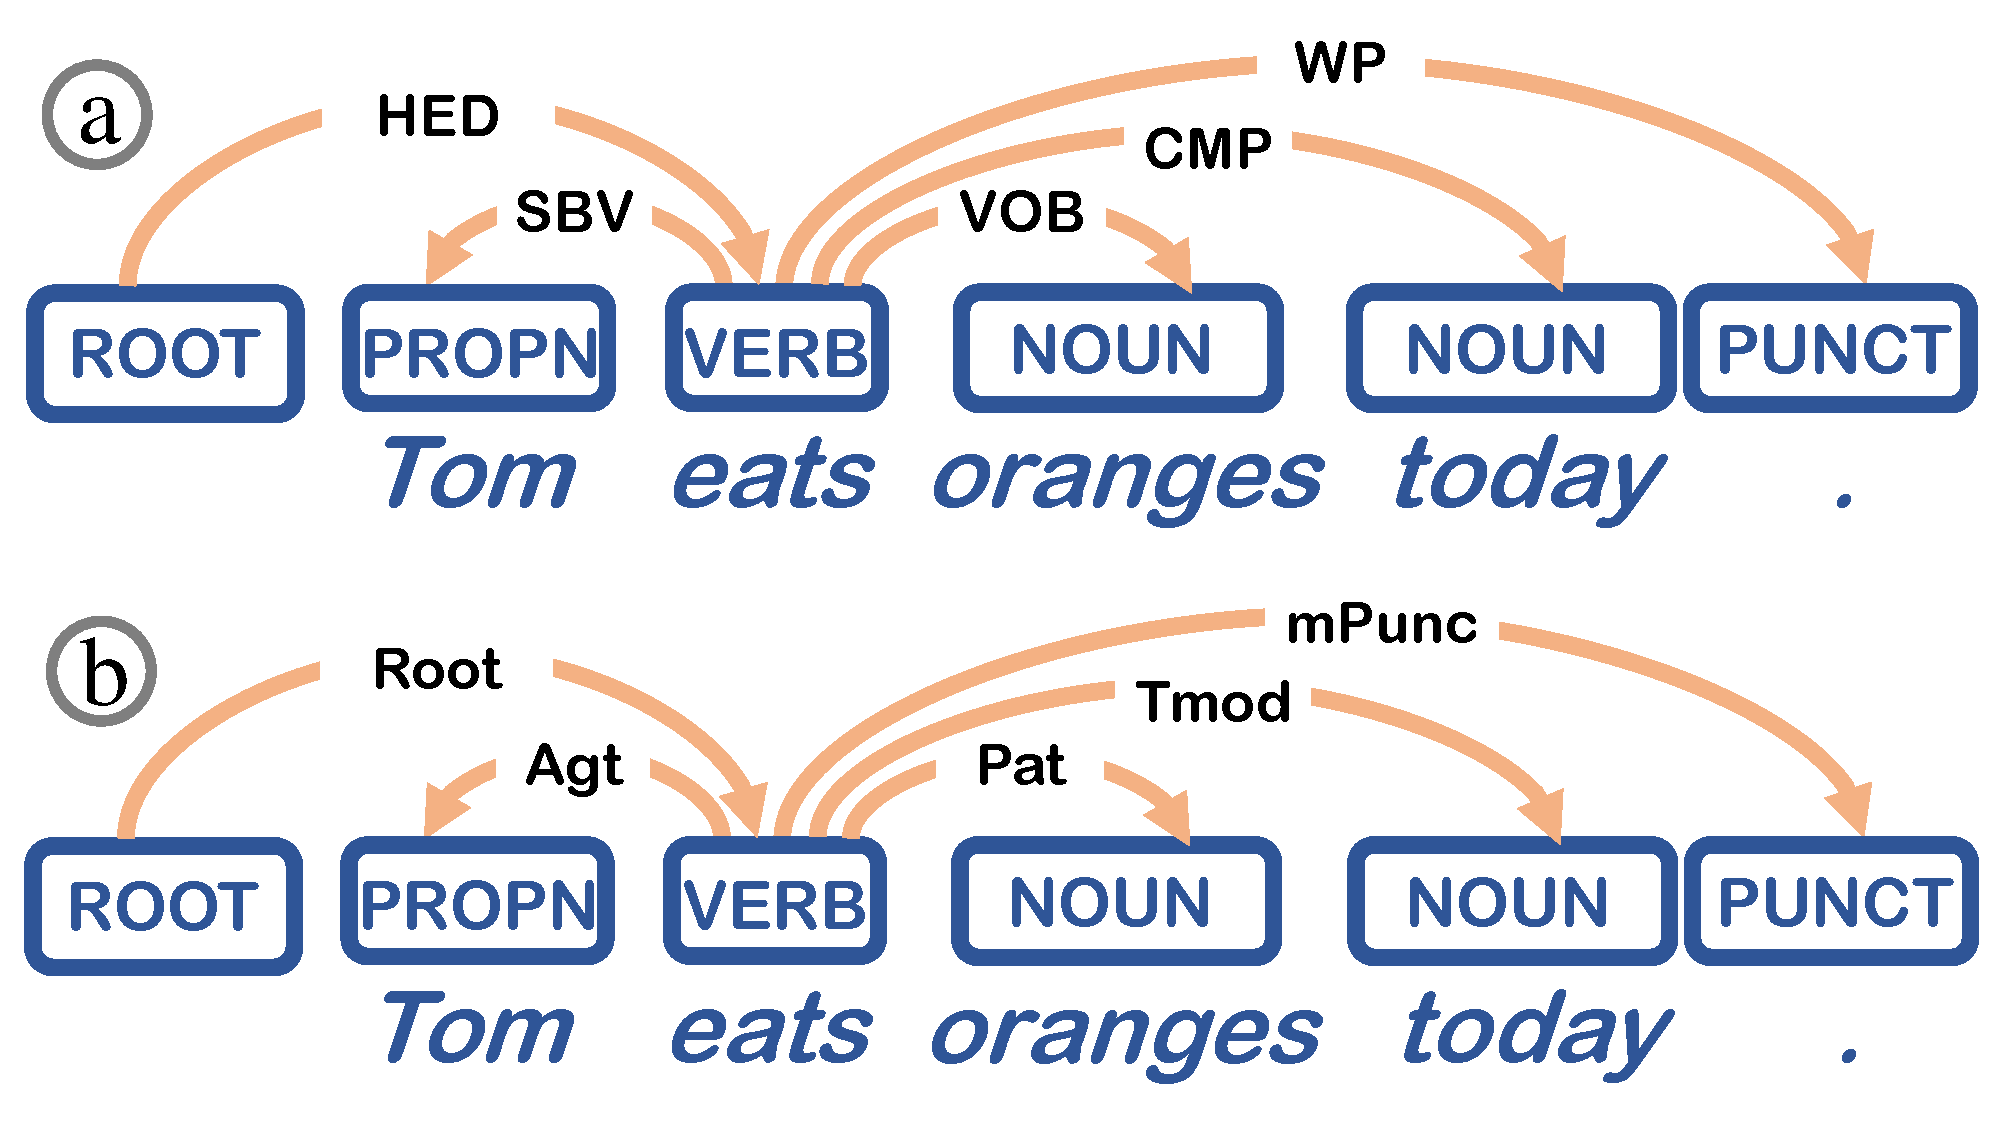
\includegraphics[width=0.48\textwidth]{Fig/dt1.pdf}
	\vspace{-0.5em}
	\caption{The dependency tree of the sentence \textit{``Tom eats oranges today."} The orange arcs refer to the type of relationship between words. In the blue box is the lexical type of the corresponding word. (a) Dependent syntactic tree.(b) Semantic dependency tree.}
	\vspace{-0.5em}
	\label{fig:DT}
\end{figure}


%    三元组抽取伪代码
\begin{algorithm}[H]
	\caption{Extracting SPO Triples}%标题
	\label{lag:EST}%标签
	\begin{algorithmic}
		\REQUIRE {A dependency syntax tree $T_{dst}$, a semantic dependency tree $T_{sdt}$, a two-dimensional array $Arr_1$ for storing triples of $T_{dst}$, a two-dimensional array $Arr_2$ for storing triples of $T_{sdt}$}
		\ENSURE  {SPO Triples}
		\STATE {\textbf{Step 1:} Use in-order traversal  for $T_{dst}$.}
		\IF {the relationship between a node and its two leaf nodes is SBV and VOB respectively}
		\STATE {store the node and its leaf nodes in $Arr_1$.}
		\ENDIF
		\STATE {\textbf{Step 2:} Use in-order traversal  for $T_{sdt}$.}
		\IF {the relationship between a node and its two leaf nodes is Agt and Pat respectively}
		\STATE {store the node and its leaf nodes in $Arr_2$.}
		\ENDIF
		\STATE {\textbf{Step 3:} Compare $Arr_1$ with $Arr_2$.}
		\IF {the same nodes exist in $Arr_1$ and $Arr_2$.}
		\STATE {combining nodes to form SPO triples.}
		\ENDIF
	\end{algorithmic}
\end{algorithm}

%在自然语言处理中,三元组抽取是一个重要的基础任务。我们借助HanLP,通过对句子的依存关系分析和语义依存分析,从而得到较好的SPO三元组。首先进行原始文本清理。一些文本数据中,尤其是文字直播评论,对句子的格式、标点符号的运用都不是特别严格。因此需要对字符、标点符号、断句空格等进行清理。然后我们借助自然语言处理的工具HanLP,对数据进行文本处理。我们使用HanLP中的依存句法分析和语义依存分析,将文本数据转换成依存关系树。依存关系分析的结果是一个有向图G=(V,A)。V代表节点,即句子中的每一个词;A代表有向边,表示词之间的依存关系。其结构通常是数据结构中的树。依存句法分析和语义依存分析都是依存关系分析的方法。前者注重句法结构,后者注重语义关联。对例句"Tom eats oranges today.",其结构如图DT所示。从中我们可以看到,依存句法树标识了语法成分,语义依存标识了语义关系。接着,根据两者的不同特性,我们可以对两者的每个节点进行遍历。从依存句法树中选取满足主谓关系(SBV)和动宾关系(VOB)的节点。从语义依存树中得到语义关系类型是“agent”还是“patient”的节点。最后将得到的节点进行对比,如果节点相同,则组合成SPO三元组。算法1中对这种方法的算法进行了详细描述。例句中,依存句法分析的结果为,SBV:eats->Tom,VOB:eats->oranges;语义依存分析的结果为,Agt:eat->Tom,Pat:eat->oranges。由此可知,该句的SPO三元组为<Tom-eats-oranges>,Tom是施者,oranges是受者。文本数据经过上述流程处理后,就可以获得具有主被动信息的SPO三元组。
In natural language processing, the triple extraction is an important fundamental task. We perform dependency analysis and semantic dependency analysis on sentences with the help of HanLP~\cite{noauthor_hanlp_nodate}, an NLP toolkit, to obtain SPO triples. First of all, raw text cleaning is performed. Some of the text data, especially the text live commentary, are not particularly strict about the formatting of sentences and the use of punctuation. Therefore, characters, punctuation marks and broken spaces need to be processed. Then we perform text processing on the data with the help of HanLP, a natural language processing tool. We use the dependency syntax analysis function and the semantic dependency analysis function in HanLP to transform the text data into a dependency tree. The result of dependency analysis is a directed graph \textit{\textbf{G=(V,A)}}. \textit{\textbf{V}} represents a node, that is, each word in the sentence; \textit{\textbf{A}} represents a directed edge, representing the dependency between words. Its structure is usually a tree. Dependency syntax analysis and semantic dependency analysis are both methods of dependency analysis. The former focuses on syntactic structure, while the latter focuses on semantic association. For the example,  \textit{``Tom eats oranges today."}, its structure is shown in Fig~\ref{fig:DT}. From this we can see that the dependency syntax tree ($T_{dst}$) identifies syntactic components, and the semantic dependency identifies semantic relations. Then, according to the different characteristics, we can traverse each node of the two. Nodes satisfying the subject-verb (\textit{SBV}) and verb-object (\textit{VOB}) relations are selected from the dependent syntactic tree. Get the nodes with semantic relationship ``Agent" (\textit{Agt}) and ``Patient" (\textit{Pat}) from the semantic dependency tree ($T_{sdt}$). Finally, the obtained nodes are compared, and if the nodes have the same value, they are combined to form the SPO triplet. A detailed description of the algorithm of this approach is given in Algorithm~\ref{lag:EST}. In the example sentence, the result of the dependency syntax analysis is, \textit{SBV}: \textit{Tom$\gets$eats}, \textit{VOB}: \textit{eats$\to$oranges}; the result of the semantic dependency analysis is, \textit{Agt}: \textit{Tom$\gets$eats}, \textit{Pat}: \textit{eat$\to$oranges}. It can be seen that the SPO triple of this sentence is $<$\textit{Tom-eats-oranges}$>$, \textit{Tom} is the possessor (\textit{PSR}), and \textit{oranges} is the possessee (\textit{PSE}). After the textual data is processed through the above process, the SPO triples with active and passive information can be obtained.

%  电影 红番区
\begin{figure*}[t]
	\centering
	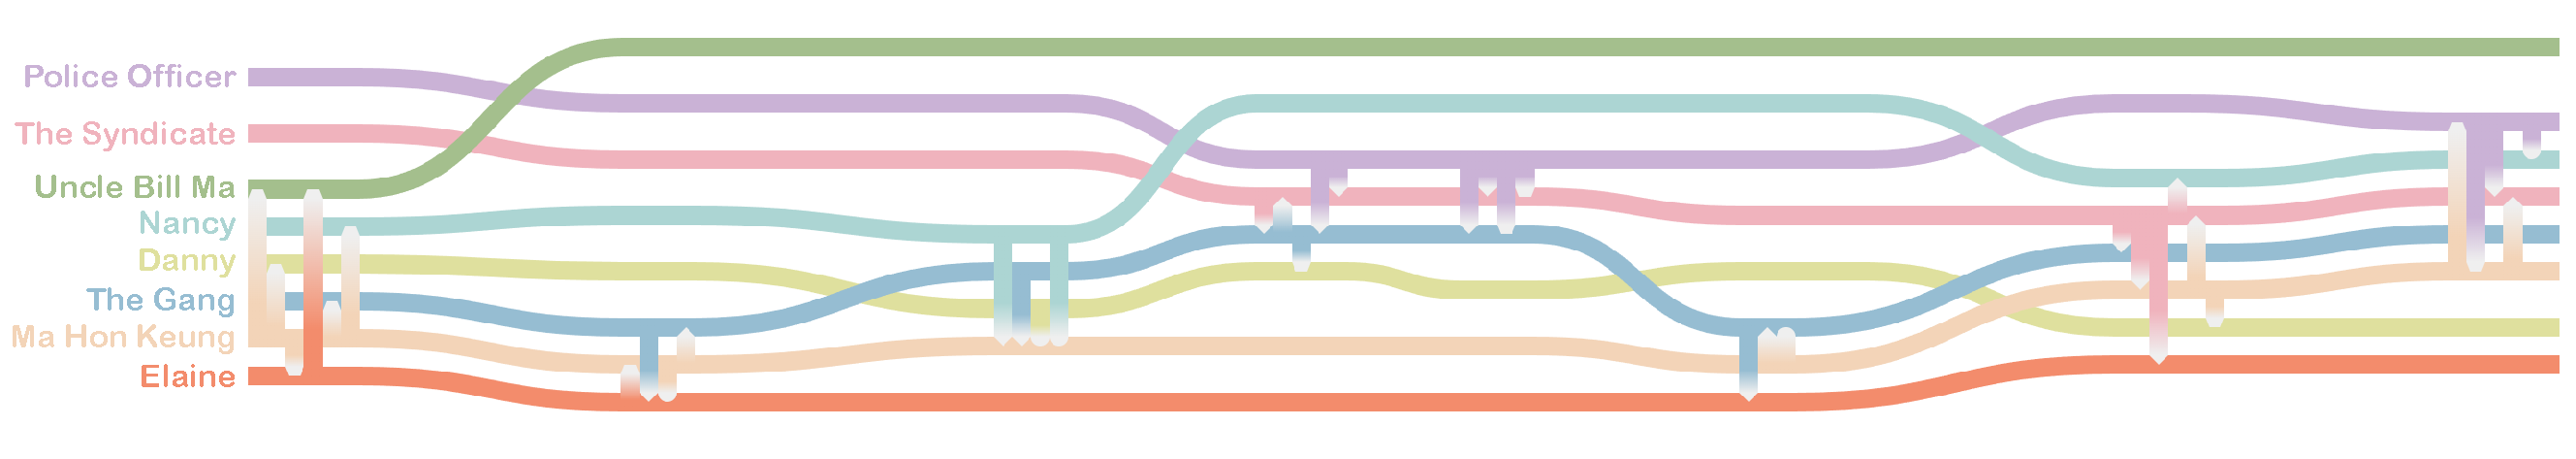
\includegraphics[width=\textwidth]{Fig/hongfanqu.pdf}
	\vspace{-2.5em}
	\caption{ Storyline visualization of the movie \textit{Rumble in the Bronx.} }
	\vspace{-0.5em}
	\label{fig:hfq}
\end{figure*}

%  电影 黑客帝国
\begin{figure*}[t]
	\centering
	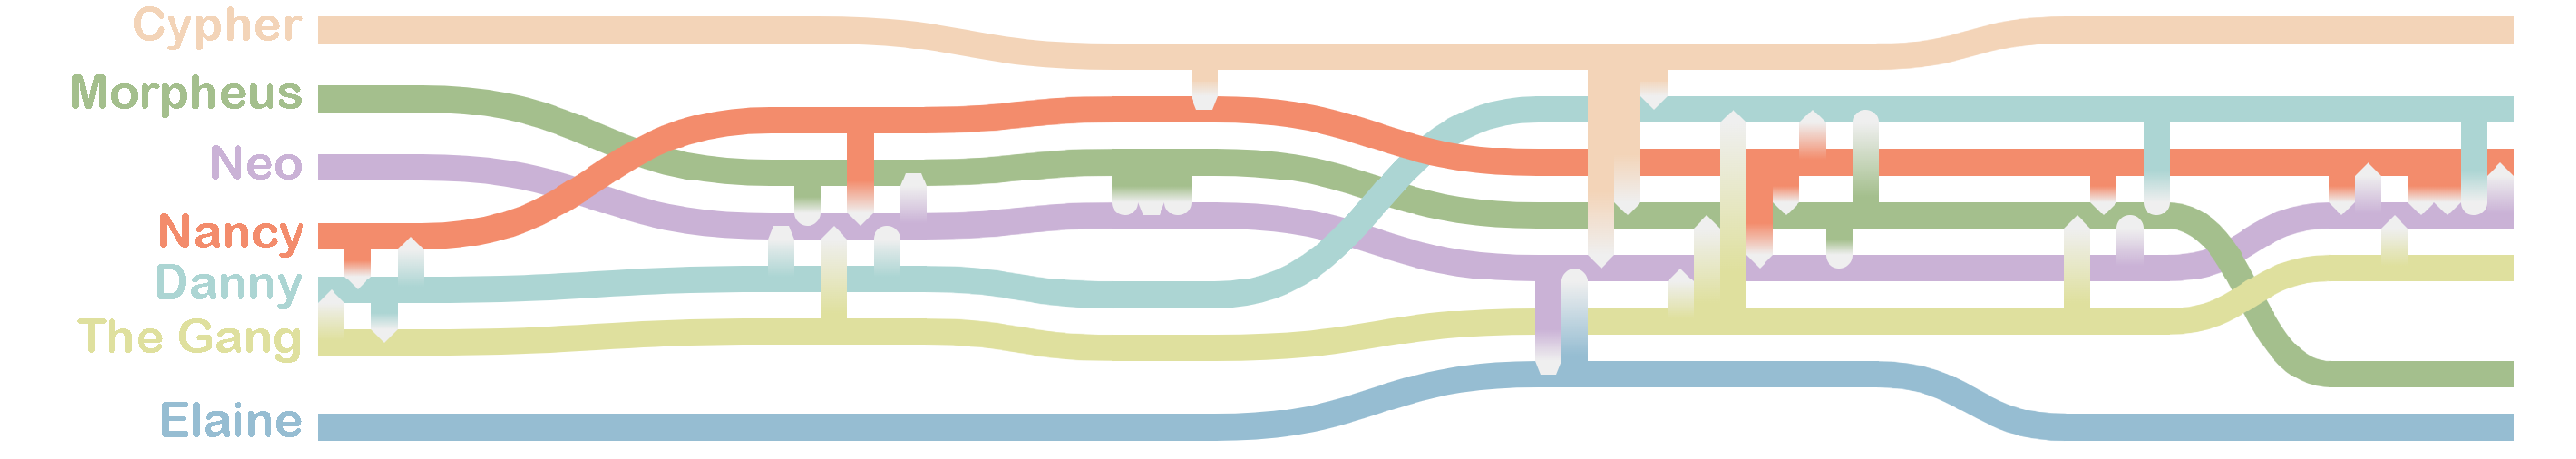
\includegraphics[width=\textwidth]{Fig/matrix.pdf}
	\vspace{-1.5em}
	\caption{Storyline visualization of the movie \textit{The Matrix}. }
	\vspace{-0.5em}
	\label{fig:matrix}
\end{figure*}

%     4.2    布局算法实现
\subsection{Layout algorithm implementation}
%遵从3.2小节提出的设计需求,我们将从选取优化目标,数学表达两个部分,详细阐述布局算法的实现。
\noindent  Following the design requirements proposed in Section 3.2, we discuss the implementation of the layout algorithm in detail from the selection of optimization objective and the mathematical expression of layout model.

%    4.2.1   选取优化目标
\subsubsection{Selection of optimization objective}
%在故事线中展示实体与实体之间关系是个新颖的尝试。现有关于故事线的工作大部分也是关于布局优化。但由于数据类型、展示意图不同,优化算法的侧重点也会大相径庭。
\noindent It is a novel attempt to show the relationship between entities in the storyline. Much of the existing work on storylines is about layout optimization. However, due to the different data types and diagrams, the focus of the optimization algorithm is quite different.

%将设计需求转换成数学问题是与提出完善的设计需求同等重要的。例如,HDR1中将每个实体编码成连续的线条,但是实体之间是离散的。因此,在同一时刻的实体位置可以转换成“分配问题”。我们的工作是围绕获得简洁、可读性强的故事线可视化展开的,换而言之就是减少故事线的复杂程度。在列举的设计需求中,SD1、SD2以及CD1,都是为此提出的。虽然SD1和SD2,分别针对的是减少点和线的复杂程度,但归根到底都是减少交点的数量。我们将线交点最少,作为优化目标1;CDR2中同一事件中的同一SPO三元组的实体尽可能靠近,作为优化目标2。综合HDR1、SDR1以及CDR2,我们将布局优化描述成多目标优化问题。
Translating design requirements into mathematical problems is as important as formulating sound design requirements. For example, each entity is encoded as a continuous line in HDR1, but the entities are discrete. Therefore, determining the physical location at the same time can be formulated as an ``\textit{Allocation Problem}". Our work aims at generating a concise, readable visualization of the storyline, in other words, our goal is reducing the confusion and complexity of the storyline. Among the design requirements listed, SDR1, SDR2 and CDR1 are all proposed for this purpose. Although SDR1 and SDR2 are aimed at reducing the complexity of points and lines, respectively, they all describe reducing the number of intersections. We take the least number of line crossings as the first optimization objective; The second optimization objective aims to guarantee the distance of the entities which belong to the same SPO triple in CDR2 are as small as possible. Incorporating HDR1, SDR1, and CDR2, we formulate the layout optimization as a multi-objective optimization problem.

%    4.2.2    数学表达
\subsubsection{Mathematical expression}
%选好优化目标,紧接着要做的是将其转换成正确的数学表达。
\noindent Once the optimization objective has been chosen, the next is to convert it into the  appropriate mathematical expression.

%op1: 可以通过比较相邻时刻实体i和j的纵坐标,来表示两条线之间是否存在交叉。我们定义yit,表示实体i在t时刻的纵坐标。如果实体i和实体j相交,则$(y_{it}-y_{jt})(y_{i,t+1}-y_{j,t+1})<0$。要使交叉点的数量最小化,优化目标1可以将表达为:
$\blacksquare $ \textbf{Line Crossing.} The existence of a cross can be indicated by comparing the vertical coordinates of entities $i$ and $j$ at adjacent moments. We define $y_{i,t}$, which denotes the longitudinal coordinate of entity $i$ at moment $t$. If there is an intersection, then $(y_{it}-y_{jt})(y_{i,t+1}-y_{j,t+1})<0$. To minimize the number of intersections, the objective function line crossings can be expressed as:

%公式1
\begin{equation}
min \quad  \frac{1}{2}\sum_{i,j}\sum_{t}\mathbb{I}_{\{(y_{i,t}-y_{j,t})(y_{i,t+1}-y_{j,t+1})<0 \}}
\end{equation}

%考虑到上述表达式中较为繁琐,我们引入Pijt和oith。两者都是0-1决策变量。前者用来判断在t时刻,第i个实体是否在第j个实体的下方。如果$y_{i,t}<y_{j,t}$,则Pijt为1,否则为0。后者用来判断实体i在时刻t在队列中的位置。如果实体i的位置为h,则oith为1,否则为0。$o_{i,t,h}$与$y_{i,t}$的数学关系可以表示成:
Considering that the above expressions are more cumbersome, we introduce $p_{i,j,t}$ and $o_{i,t,h}$. Both of them are 0-1 decision variables. The former is used to determine whether the entity $i$ is below the entity $j$ at moment $t$. $p_{i,j,t}$ is 1 when $y_{i,t}<y_{j,t}$, otherwise it is 0. The latter is used to determine the position of entity $i$ in the queue at moment $t$. Then $o_{i,t,h}$ is 1 when the position of entity $i$ is $h$, otherwise it is 0. The mathematical relationship between $o_{i,t,h}$ and $y_{i,t}$ is expressed as:

%公式2
\begin{equation}
y_{i,t} =  \sum_{h}o_{i,t,h}h \quad\quad
\end{equation}


%$O_{i,t,h}$和$P_{i,j,t}$之间的数学关系可以表示为:
\noindent The mathematical relationship between $o_{i,t,h}$ and $p_{i,j,t}$ is expressed as:

%公式3
\begin{equation}
p_{i,j,t} = 1, \quad\quad when\quad o_{i,t,h_1} + o_{j,t,h_2}=2\;\&\;h_1<h_2
\end{equation}

%至此,我们可以将公式(1)简化为:
\noindent Using $p_{i,j,t}$, we can simplify Eq.(1) as:

%公式4
\begin{equation}
min \quad \sum_{i,j,t}p_{i,j,t}p_{j,i,t+1}
\end{equation}

%op2: 对op2,我们可以把它转述为,在同一时刻t,有联系的两个实体i和j之间的纵坐标差值最小。为了指定适用的实体,减少计算量,我们引入两个0-1常量,$C_{i,e}$和$B_{e,t}$。$C_{i,e}$指实体i参与了事件e。$B_{e,t}$指t时刻发生的是事件e。在数学上说,op2可以表达为:
$\blacksquare$ \textbf{Entity Distance.} We can formulate it as, the difference in vertical coordinates between two entities $i$ and $j$ that are connected has the smallest value at the same moment $t$. To specify the applicable entities and reduce the computational effort, we introduce two 0-1 constants, $C_{i,e}$ and $B_{e,t}$. $C_{i,e}$ means that entity $i$ is involved in event $e$. $B_{e,t}$ means that it is event $e$ that occurs at moment $t$. Mathematically speaking, the objective function can be expressed as:

%公式5
\begin{equation}
min \quad \sum_{i,j,t,e}(\sum_{h}o_{i,t,h}\cdot h-\sum_{h}o_{j,t,h}\cdot h)^2B_{e,t}C_{i,e}C_{j,e}
\end{equation}

%将op1和op2结合,就可以得到完整的多目标优化方程。$\alpha$ 和 $\beta$是多目标优化方程求解时的权重。在经过多次实验后,我们将$\alpha$ 和 $\beta$的值分别设置为1和0.2。
The complete objective function of multi-objective optimization model can be obtained as Eq.(3) and Eq.(4). We utilize a weighted linear combination to convert the above two objective function as followings:

\vspace{-1em}
%公式6
\begin{equation}
\begin{split}
min \quad &\alpha\sum_{i,j,t}p_{i,j,t}p_{j,i,t+1} + \\
&\beta\sum_{i,j,t,e}(\sum_{h}o_{i,t,h}\cdot h-\sum_{h}o_{j,t,h}\cdot h)^2B_{e,t}C_{i,e}C_{j,e}
\end{split}
\end{equation}
where $\alpha$ and $\beta$ are the weights to balance the importance of two objective function. After several experiments, we set the values of $\alpha$ and $\beta$ as 1 and 0.2.

%首先写的是指派问题
%约束:首先,我们将实体的排序转换为“指派问题”。假设我们有$H$个箱子组成的队列,在t时刻,实体i必须且只能进一个箱子$h$。为了将该问题转换成数学表达式,我们可以使用变量$O_{i,t,h}$和$P_{i,j,t}$,h1和h2分别为实体i和j在t时刻在队列中的位置。“指派问题”可以表达为:
$\blacksquare$ \textbf{Constraints:} First, we model the ordering of entities as an ``\textit{Assignment Problem}". Hypothetically, we have a queue of $H$ boxes and at time $t$, entity $i$ must and can enter only the box $h$. To convert this problem into a mathematical expression, we can use the variables $o_{i,t,h_1}$ and $o_{j,t,h_2}$, where $h_1$ and $h_2$ are the positions of entities $i$ and $j$. These following constraints are employed to guarantee the uniqueness of entities and locations:

\vspace{-1em}
%公式7
\begin{subequations}
	\begin{align}
	\sum_io_{i,t,h}&=1, \quad\quad \forall t,h \\
	\sum_ho_{i,t,h}&=1, \quad\quad \forall i,t \\
	p_{i,j,t}+p_{j,i,t}&=1, \quad\quad \forall t,i,j\;\&\;i \neq j\\
	p_{i,j,t}&=0, \quad\quad \forall t,i=j
	\end{align}
\end{subequations}

%公式(7a)确保对每个实体$i$,在任意的t时刻,只可以在队列中占据一个位置。公式(7b)确保在任意的t时刻,队列中没有空的位置。公式(7c)和(7d)确保在相同的t时刻实体i和j之间存在位置上的差异,同时排除了只取到一个实体的情况。
\noindent Eq.(7a) ensures that for each entity $i$, at any moment $t$, only one position in the queue can be occupied. Eq.(7b) ensures that at any moment $t$, there are no empty positions in the queue. Eq.(7c) and Eq.(7d) ensure that there is a difference in position between entities $i$ and $j$ at the same moment $t$, while excluding the case where only one entity is taken.

%在实体进行排序的同时,我们需要对参与同一事件e的实体进行约束。正如CDR1中所提及的,在事件e的持续时间Te内 ,实体的纵坐标位置保持不变。如图5。a中所示。其数学表达式为:
While the entities are sorted, we need to constrain the entities involved in the same event $e$. As mentioned in CDR1, during the time interval $T_e$ of the event $e$ , the position of the vertical coordinate of the entity remains unchanged. As shown in Fig~\ref{fig:EG}.(a), the mathematical expression is: 

\vspace{-1em}
%公式8
\begin{equation}
o_{i,t_1,h}=o_{i,t_2,h}, \quad\quad when \quad C_{i,e}=B_{e,t_1}=B_{e,t_2}=1 \;\&\; t_1,t_2 \in T_e
\end{equation}

%当$C_{i,e}$=1时,表示实体i参与了事件e;当$B_{e,t1}=$B_{e,t2}$=1时,表示在事件e发生在时刻$t_1$和$t_2$
\noindent where $C_{i,e}=1$, indicating that entity $i$ is involved in event $e$; $B_{e,t1}=B_{e,t2}=1$, indicating that at event $e$ occurs at both moments $t_1$ and $t_2$.

%EG的示意图。
\begin{figure}[h]
	\begin{minipage}[t]{0.3\linewidth}
		\flushright
		\vspace{0em}
		\centerline{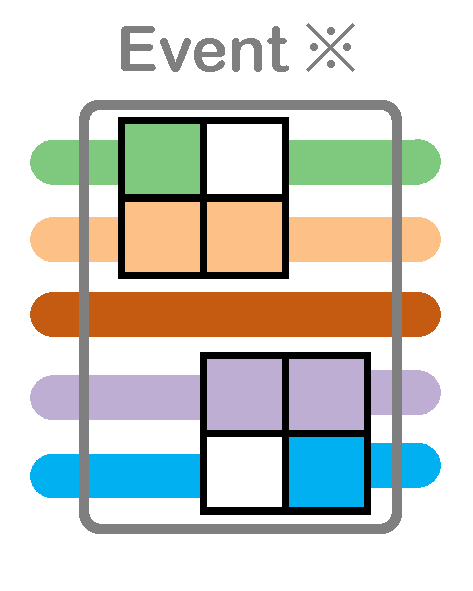
\includegraphics[width=1in,height=3.5cm]{Fig/BadEG.pdf}}
		\vspace{-0.5em}
		\caption{Events$\divideontimes$ are represented by two separate pixel maps.}
		\label{fig:BadEG}
		\vspace{-0.5em}
	\end{minipage}
	\hspace{.2in}
	\begin{minipage}[t]{0.6\linewidth}
		\flushright
		\vspace{-1em}
		\centerline{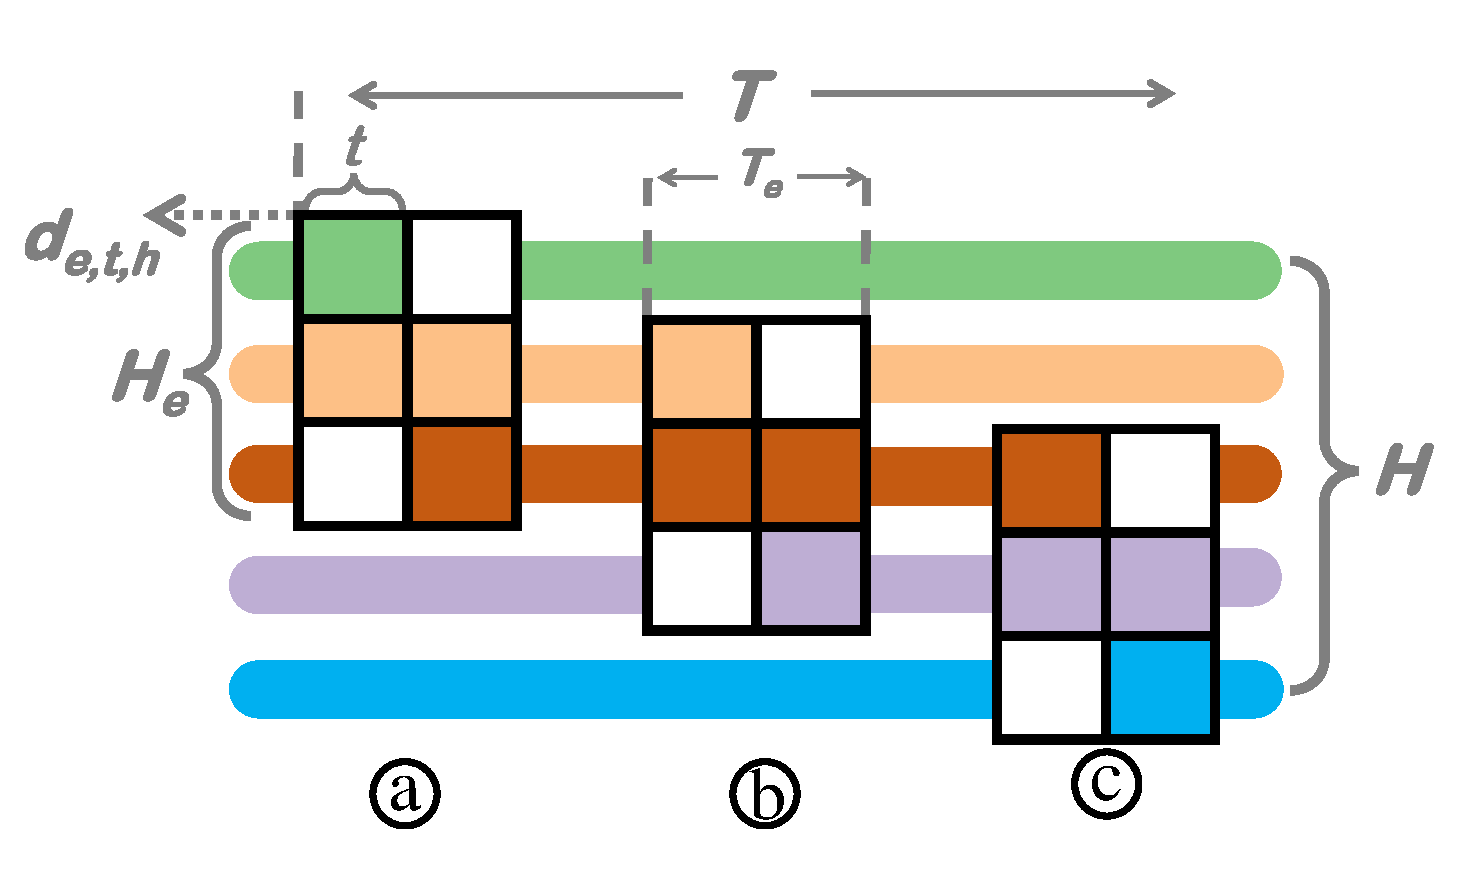
\includegraphics[width=2.4in,height=4cm]{Fig/EG.pdf}}
		\vspace{-1em}
		\caption{Diagram of ``\textit{Sliding Window}". The state of the window during sliding: (a) at the start of the entity queue, (b) in the queue, (c) at the end of the queue.}
		\label{fig:EG}
		\vspace{-0.5em}
	\end{minipage}
\end{figure}

%在实验中我们发现,只有公式7和8时会发生图4中所示的错误。灰色框为事件※,其可视化结果应该与图5.a类似,但事实上变成了两个独立的像素图。这意味着原本应该依次靠在一起的实体组内进入了一个不参与该事件的实体,即棕色实体。因此,我们需要对参与同一事件e的实体组在纵轴上进行约束。
After several experiments, we found that the error shown in Fig~\ref{fig:BadEG} would occur with only constraints of Eq.7 and Eq.8. The gray box represents the Event$\divideontimes$, which should be visualized similarly to Fig~\ref{fig:BadEG}, but in fact turns out to be two separate pixel maps. An entity that is not involved in the Event$\divideontimes$, the brown one, is inserted in the group of entities that should have been leaning together in order. Therefore, we need to constrain the group of entities involved in the same event $e$ on the vertical axis.

%为了使参与同一事件的实体组中间不插入无关实体,可以将该实体组看成一个窗口,其长度为$H_e$。实体组的位置调整可以视为“滑动窗口”。我们引入了$d_{e,t,h}$,它是一个0-1决策变量量,用来确定在时刻t发生的事件e中参与的实体组成的窗口的起点。当窗口滑动时,存在以下几种情况。窗口的起始点是实体队列的起点;窗口在实体队列中;窗口的终点是实体队列的终点。如图5所示,(a),(b),(c)分别对应三种情况。
To keep the group of entities involved in the same event from inserting irrelevant entities, the entity group can be considered as a window with the length $H_e$. The adjustment of the position of the entity group can be considered as a ``\textit{Sliding Window}" problem. We define $d_{e,t,h}$, which is a 0-1 decision variable that determines the starting point of the window consisting of the entities involved in event $e$ at moment $t$. When the window is sliding, there are several cases as follows. The start of the window is the start of the queue of entities; the window is in the queue of entities; and the end of the window is the end of the queue of entities. As shown in Fig~\ref{fig:EG}.(a), Fig~\ref{fig:EG}.(b), and Fig~\ref{fig:EG}.(c) correspond to the three cases, respectively.

\vspace{-1em}
%公式9
\begin{subequations}
	\begin{align}
	\sum_{h=0}^{H-H_e}d_{e,t,h}&=1, \quad\quad \forall e,t\;\; when\;\; B_{e,t} = 1\\
	\sum_{h=H-H_e+1}^{H-1}d_{e,t,h}&=0, \quad\quad \forall e,t\;\; when\;\; B_{e,t} = 1\\
	\sum_{i=0}^{H}\sum_{h_b=0}^{h-1}o_{i,t,h_b}C_{i,e}&=0, \quad\quad \forall e,t \;\;when\;\; d_{e,t,h}=1 \\
	\sum_{i=0}^{H}\sum_{h_e=h}^{h+H_e-1}o_{i,t,h_e}C_{i,e}&=H_e, \quad\quad \forall e,t \;\;when\;\; d_{e,t,h}=1
	\end{align}
\end{subequations}

%公式(9)详细描述了解决上述问题的算法。公式(9a)保证了当$h\in [0,\;H-H_e]$时,存在一个位置为窗口的起始点。公式(9b)保证了当$h\in [H-H_e+1,H-H-1]$时,不存在窗口的起始点。公式(9b)保证了不会发生溢出情况。公式(9a)及(9b)保证了当$h\in[0, H-1]$时有且仅有一个点为窗口起始点。公式(9c)可以确保参与事件$e$的实体$i$不可能排在起始点$h$前。公式(9d)可以确保参与事件$e$的实体都在窗口内。
Eq.9 describes the constraints of ``\textit{Sliding Window}". Eq.(9a) ensures that there exists a location for the start of the window when $h\in [0,\;H-H_e]$. Eq.(9b) ensures that there is no starting point for the window when $h\in [H-H_e+1,H-H-1]$. Eq.(9b) ensures that no overflow occurs. Eq.(9a) and (9b) together guarantee that there is one and only one pointis the window start point when $h\in[0, H-1]$. Eq.(9c) ensures that the entity $i$ involved in the event $e$ cannot be ranked in front of the starting point $h$. Eq.(9d) can ensure that the entities involved in the event $e$ are within the window.

%经过“实体间关系提取”和“多目标优化算法建模”后,我们将数据和求解模型输入数学求解工具Gurobi,得到全局最优解。
After ``inter-entity relationship extraction" and ``multi-objective optimization algorithm modeling", we input the data and optimization model into \textit{Gurobi}~\cite{noauthor_gurobi_nodate}, a mathematical solution tool, to obtain the global optimal solution.

%    5     关系展示 本节主要讲relation的表现方式。
\section{RELATIONSHIP DISPLAY}
%在本章节,我们主要介绍实体关系的设计。首先,为了设计有效的视觉元素来映射实体间关系,我们在一定的限制框架下开展了一次头脑风暴。经过分析和总结,我们最终确定了12种设计方案。然后,我们综合分析这些案例,提出了一种设计空间。最后,我们执行了一项用户调研来收集相关评价。
\noindent In this section, we mainly introduce the design of entities relationship. Firstly, in order to design effective visual elements to map the relationships between entities, we conducted a brainstorming under certain restrictive framework. After analysis and summary, we finally settled on 12 design schemes. Then, we comprehensively analyze these options and propose a design space. Finally, we conducted a user study to collect relevant reviews.
%    5.1    %设计案例
\subsection{Design Scheme}
% 我们邀请了可视化领域的3位硕士研究生和1位博士研究生进行了一场关于实体关系视觉表达的头脑风暴。经过分析和讨论,我们收集到数份设计图。我们对这些设计方案进行归纳总结后,得到了如下3种图例:箭头,基础图形和渐变。这些图例中都存在指向性的标识,即关系中的"施者->受者"。在箭头图例中,方向由箭头来隐喻;在基础图形中,方向由图形朝向来隐喻;在颜色渐变中,方向由颜色从深向浅过度来隐喻。
\noindent We invited three master students and one PhD student in the field of visual analysis to conduct a brainstorming on the visual representation of entities relationship. After analysis and discussion, we collected several design schemes. After summarizing these design schemes, we identified three types of legends that can represent entities relationships, and there is a directional identification in these legends, that is, ``\textit{giver} $\rightarrow$ \textit{receiver}" in the SPO triples.

\ding{172} Directed arrow:  `` \raisebox{-0.75mm}{
\includegraphics[scale=0.15]{Fig/arrow.png}} ", the direction is metaphorically represented by the arrow.

\ding{173} Basic shape: `` \raisebox{-0.75mm}{
\includegraphics[scale=0.015]{Fig/bg4.png}} ", `` \raisebox{-0.75mm}{
\includegraphics[scale=0.15]{Fig/bg2.png}} ", `` \raisebox{-0.75mm}{
\includegraphics[scale=0.15]{Fig/bg3.png}} ", the direction is metaphorically represented by the orientation of the graphics.

\ding{174} Color gradient: ``\raisebox{-0.75mm}{
\includegraphics[scale=0.15]{Fig/jianbian.png}}", the direction is metaphorically represented by the transition of color from dark to light.

%经过参与者的讨论,我们发现,上述图例之间的组合形成的效果也很好。例如将箭头与基础图形结合可以得到:···;同理,将基础图形与颜色渐变结合可以得到:···。我们综合上述图例制作了下述12个设计案例:
After the discussion among the participants, we found that the combination of the above legends also has a good effect in expressing the entity relationship. 

\ding{175} Hybridizing the Directed arrow with the Basic shape yields: `` \raisebox{-1mm}{
\includegraphics[scale=0.015]{Fig/mixabg4.png}} ", `` \raisebox{-1mm}{
\includegraphics[scale=0.15]{Fig/mixabg3.png}} ".

\ding{176} Hybridizing the Basic shape with the Color gradient yields: `` \raisebox{0mm}{
\includegraphics[scale=0.015]{Fig/mixcbg4.png}} ", `` \raisebox{-1mm}{
\includegraphics[scale=0.15]{Fig/mixcbg2.png}} ", `` \raisebox{-1mm}{
\includegraphics[scale=0.15]{Fig/mixcbg3.png}} ".



%案例
\begin{figure}[h]
	\vspace{-0.5em}
	\begin{minipage}{0.24\linewidth}
		\centerline{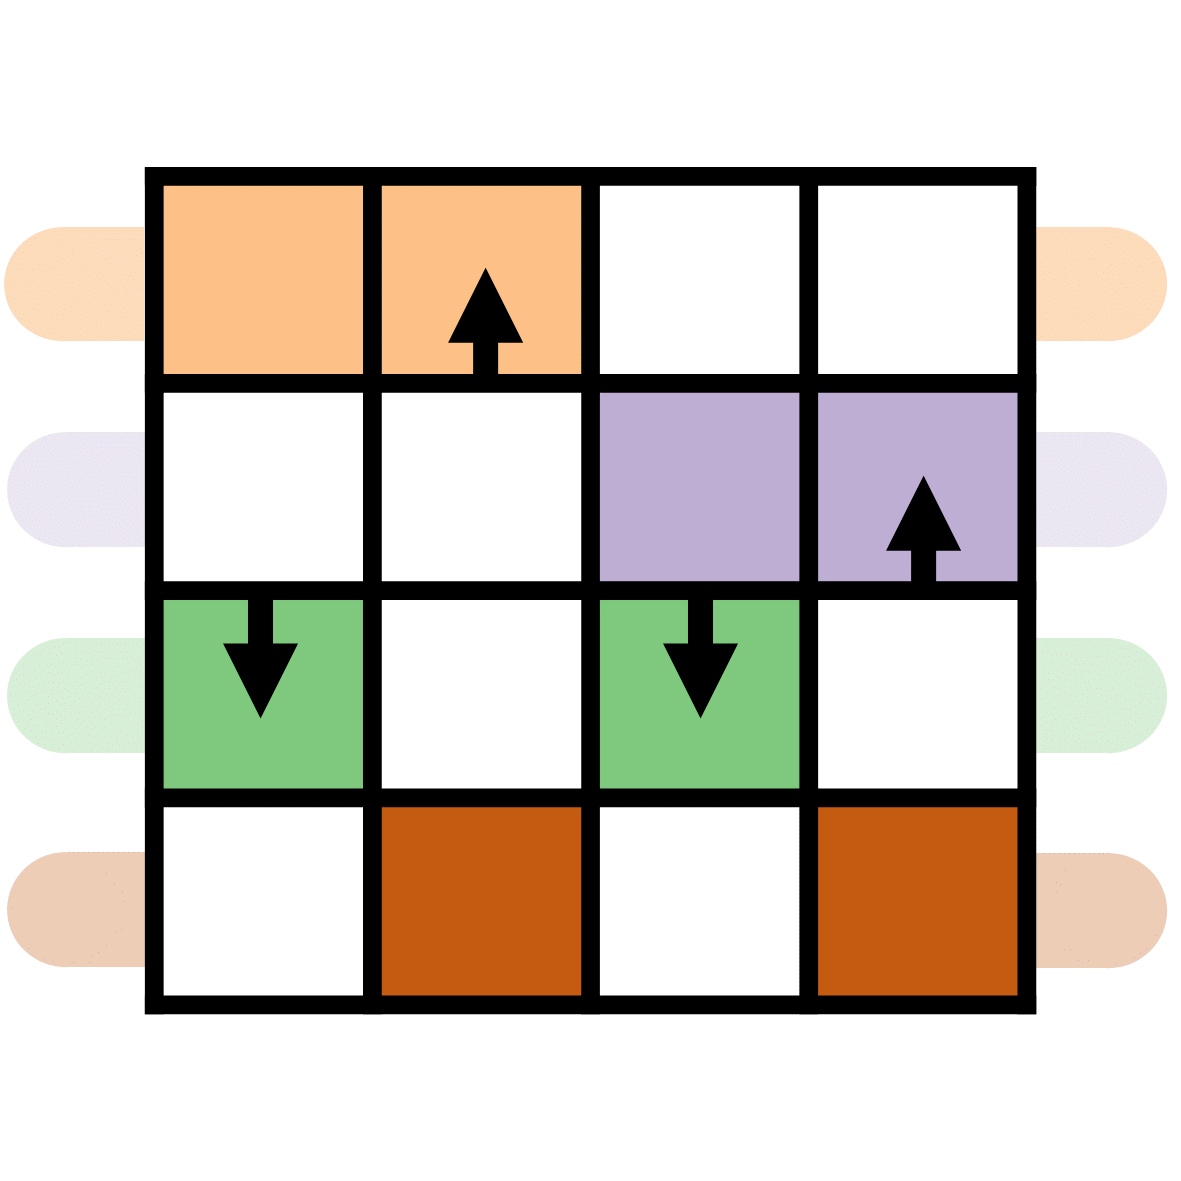
\includegraphics[width=\textwidth]{Fig/11.png}}
		\vspace{-1pt}
		\centerline{(a).1}
		\centerline{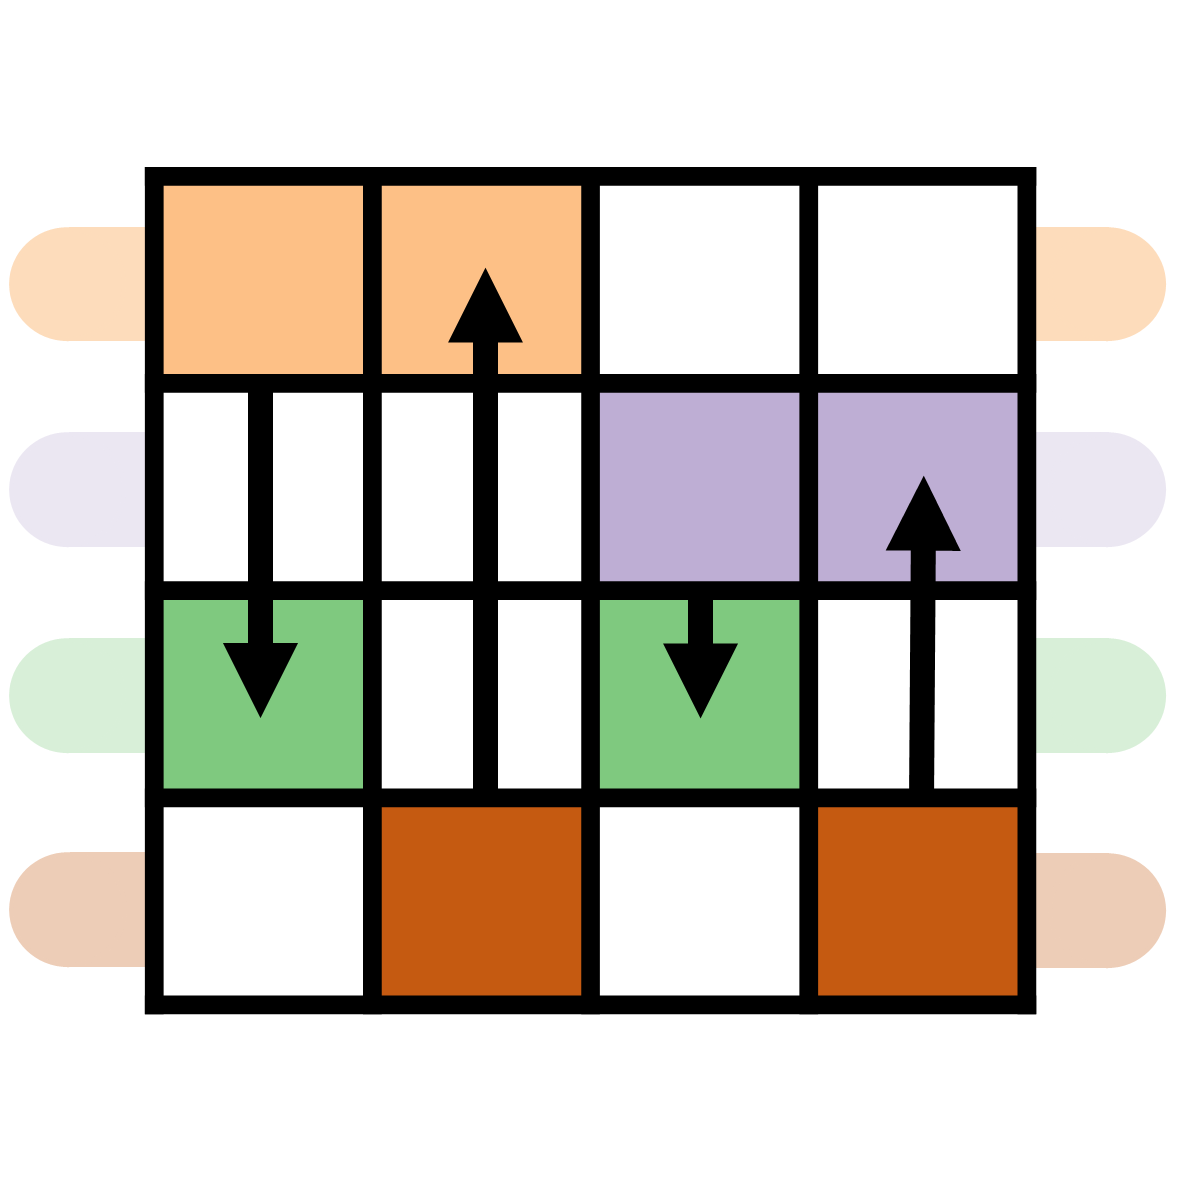
\includegraphics[width=\textwidth]{Fig/12.png}}
		\vspace{-1pt}
		\centerline{(a).2}
		\centerline{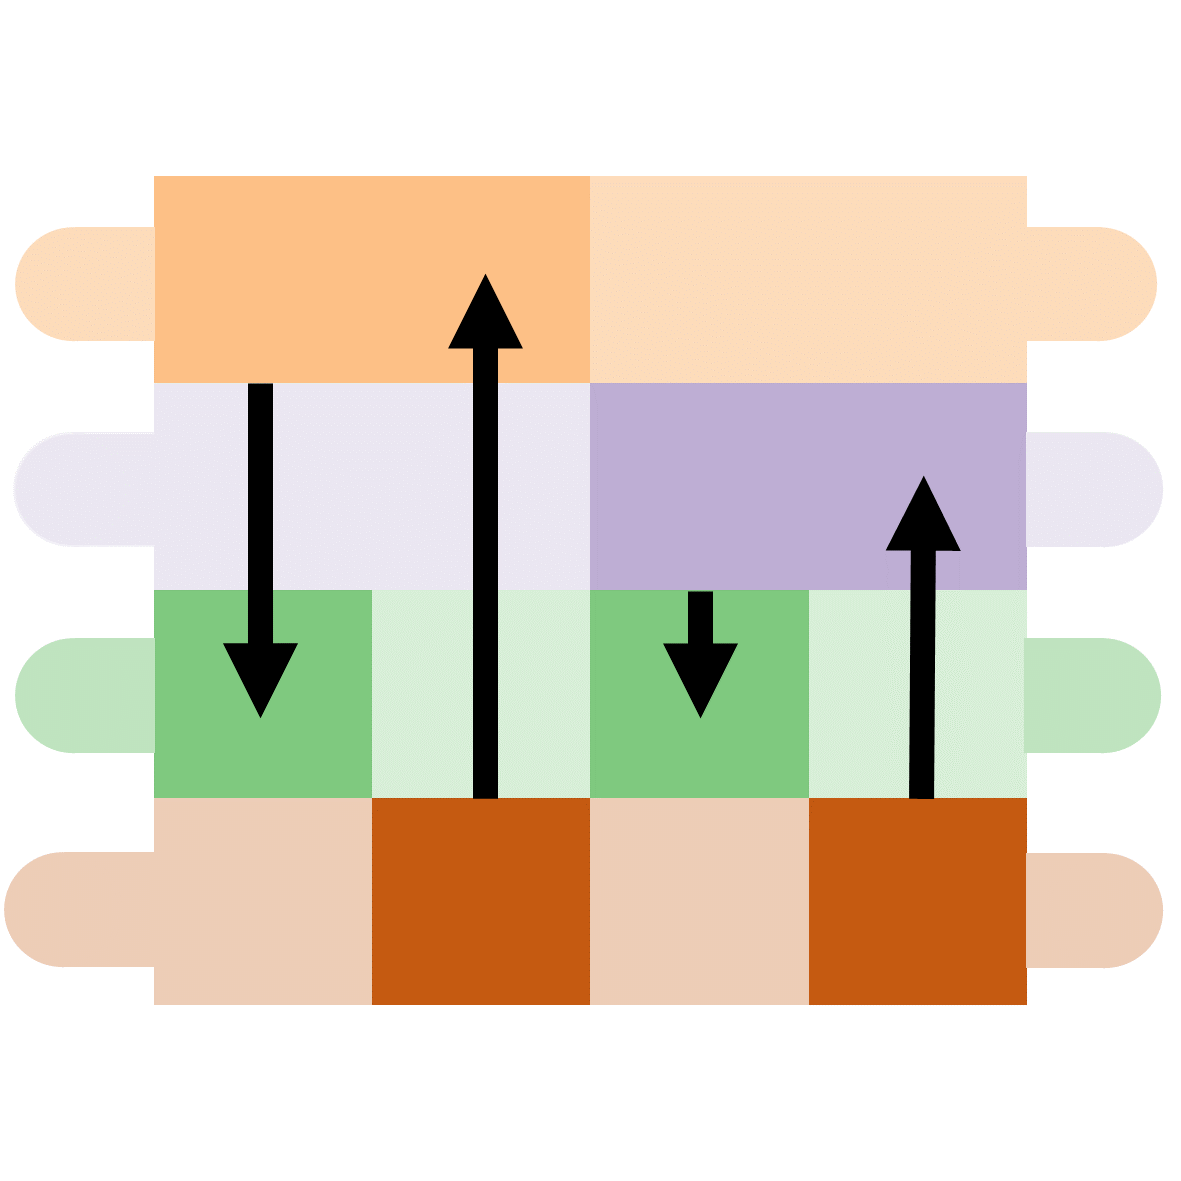
\includegraphics[width=\textwidth]{Fig/13.png}}
		\vspace{-1pt}
		\centerline{(a).3}
	\end{minipage}
	\begin{minipage}{0.24\linewidth}
		\centerline{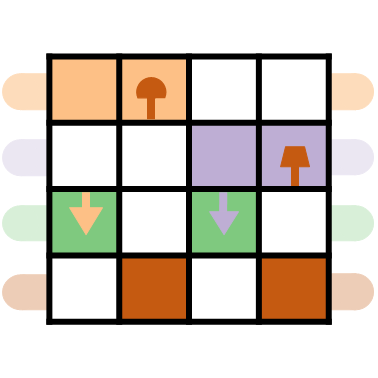
\includegraphics[width=\textwidth]{Fig/21.png}}
		\vspace{-1pt}
		\centerline{(b).1}
		\centerline{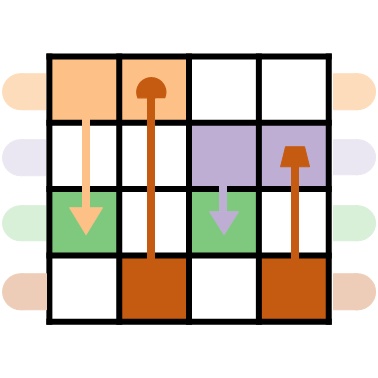
\includegraphics[width=\textwidth]{Fig/22.png}}
		\vspace{-1pt}
		\centerline{(b).2}
		\centerline{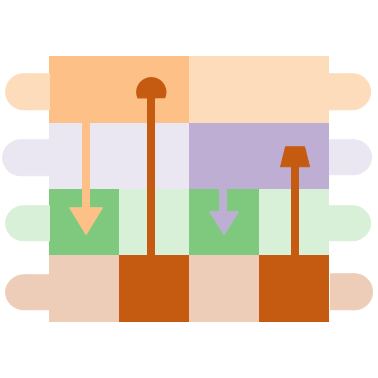
\includegraphics[width=\textwidth]{Fig/23.png}}
		\vspace{-1pt}
		\centerline{(b).3}
	\end{minipage}
	\begin{minipage}{0.24\linewidth}
		\centerline{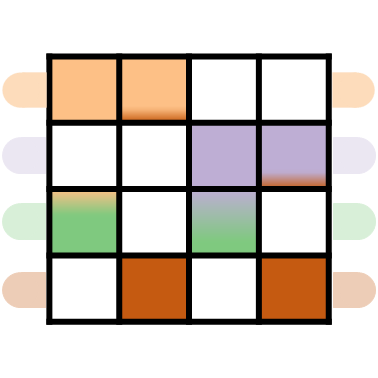
\includegraphics[width=\textwidth]{Fig/31.png}}
		\vspace{-1pt}
		\centerline{(c).1}
		\centerline{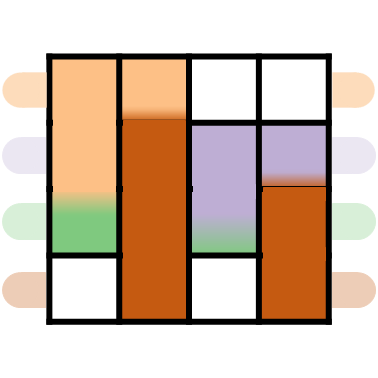
\includegraphics[width=\textwidth]{Fig/32.png}}
		\vspace{-1 pt}
		\centerline{(c).2}
		\centerline{
\includegraphics[width=\textwidth]{Fig/33.png}}
		\vspace{-1pt}
		\centerline{(c).3}
	\end{minipage}
	\begin{minipage}{0.24\linewidth}
		\centerline{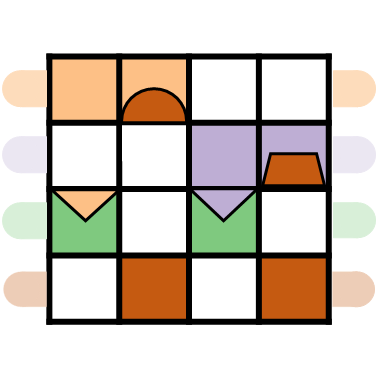
\includegraphics[width=\textwidth]{Fig/41.png}}
		\vspace{-1pt}
		\centerline{(d).1}
		\centerline{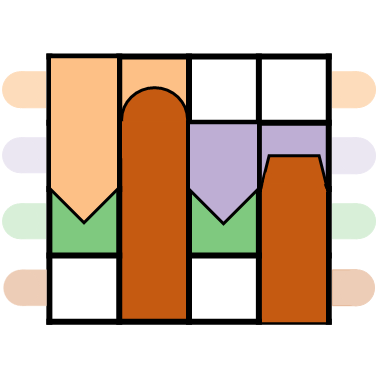
\includegraphics[width=\textwidth]{Fig/42.png}}
		\vspace{-1pt}
		\centerline{(d).2}
		\centerline{
\includegraphics[width=\textwidth]{Fig/43.png}}
		\vspace{-1pt}
		\centerline{(d).3}
	\end{minipage}
	\caption{Design schemes. (a)Directed arrow; (b)Directed arrow + Basic shape; (c)Color gradient; (d)Color gradient + Basic shape.}
	\label{fig:DC}
	\vspace{-0.5em}
\end{figure}

%图7为实体关系的设计案例。图7.a中的图例为箭头,图7.b中的图例为箭头+基础形状,图7.c中的图例为颜色渐变,图7.d中的图例为基础形状+颜色渐变。我们提出了一个设计空间,用来评判设计案例的功能。设计空间中的评价原则有:\ding{183}是否能展示实体间具有关系,\ding{184}是否能区分关系的施者与受者,\ding{185}是否能展示关系属性。如表格所示,设计方案(a)和(c)在部分功能上稍显欠缺,设计方案(b)和(d)能满足上述所有功能。
Fig~\ref{fig:DC} shows design schemes of entities ralationship, where the legends used are Arrow, Arrow + Basic shape, Color gradient, and Basic shape + Color gradient. We propose a design space for judging the functionality of each design scheme. The evaluation principles in the design space are: \ding{182} whether the entity relationship can be demonstrated, \ding{183} whether the giver and the receiver of the relationship can be distinguished, and \ding{184} whether the relationship properties can be demonstrated. As shown in Tab~\ref{tab:jf}, designs scheme (a) and (c) in Fig~\ref{fig:DC} are slightly lacking in some functions, while designs scheme (b) and (d) in  Fig~\ref{fig:DC} are able to satisfy the above functions.

%表格1绘制
\renewcommand{\arraystretch}{1.2}
\newcolumntype{Y}{>{\centering\arraybackslash}X}
\begin{table}[h]
	\caption{Judging the functionality of each design Scheme}
	\centering
	\begin{tabularx}{0.45\textwidth}{| c | Y | Y | Y | Y |}
		\hline
		\multicolumn{2}{|c|}{\multirow{2}{*}{Design Scheme}} & \multicolumn{3}{c|}{Evaluation Metrics}  \\
		\cline{3-5}
		\multicolumn{2}{|p{1cm}|}{\centering}
		& \ding{182} & \ding{183} & \ding{184}    \\
		\hline
		\multirow{3}{*}{Directed arrow} {\centering}
		& 1    & \checkmark &   &                          \\
		\cline{2-5}
		& 2    & \checkmark & \checkmark &                          \\
		\cline{2-5}
		& 3    & \checkmark & \checkmark &                          \\
		\hline
		\multirow{3}{*}{\makecell{Directed arrow +\\Basic shape}}
		& 1    & \checkmark & \checkmark & \checkmark                        \\
		\cline{2-5}
		& 2    & \checkmark & \checkmark & \checkmark                        \\
		\cline{2-5}
		& 3    & \checkmark & \checkmark & \checkmark                        \\
		\hline
		\multirow{3}{*}{\makecell{Color gradient} }
		& 1    & \checkmark & \checkmark &                          \\
		\cline{2-5}
		& 2    & \checkmark & \checkmark &                          \\
		\cline{2-5}
		& 3    & \checkmark & \checkmark &                          \\
		\hline
		\multirow{3}{*}{\makecell{Color gradient\\+ Basic shape} }
		& 1    & \checkmark & \checkmark & \checkmark                        \\
		\cline{2-5}
		& 2    & \checkmark & \checkmark & \checkmark                        \\
		\cline{2-5}
		& 3    & \checkmark & \checkmark & \checkmark                        \\
		\hline
	\end{tabularx}
	\label{tab:jf}
\end{table}

%用户调研   23人有数据分析方面的实践经历,3人从事计算机视觉的相关研究,21人熟悉数据可视化。除了了解参与者的个人信息外,我们确保所有受试者没有色盲或者色弱方面的视觉认知障碍,在理解视觉映射方面也没有困难
%     5.2    用户调研
\subsection{User Study}
%图例除了要满足尽可能多的功能外,也要兼备美学和可理解性。因此,为了评估上述设计方案,我们通过调查问卷的方式对25名受试者进行了调研。其中4名参与者为本科生,21名参与者为研究生。我们分别向受试者展示了图6中的(a),(b),(c),(d)四组设计方案,要求受试者根据个人主观,在每组中选择最喜欢的一个设计方案。最后参与者们再被要求,选出最终的设计方案。相关统计结果如下图所示。
\noindent In addition to satisfying as many functions as possible, legends also need to be both aesthetically pleasing and understandable. Therefore, in order to evaluate the above design, we investigated twenty-five participants by means of a questionnaire. Four of the participants were undergraduate students and twenty-one of participants were graduate students. We presented the participants with the four groups of design schemes (a), (b), (c), and (d) in Fig~\ref{fig:DC} respectively. We asked the participants to choose the most preferred design scheme in each group according to their personal subjectivity. Participants subjectively selected the most preferred in each group after observation. Finally, the participants were asked to compare and select the final design scheme. The relevant statistical results are shown in Fig~\ref{fig:sta} below.

%图8用户统计数据
\begin{figure}[h]
	\centering
	\vspace{-1.2em}
	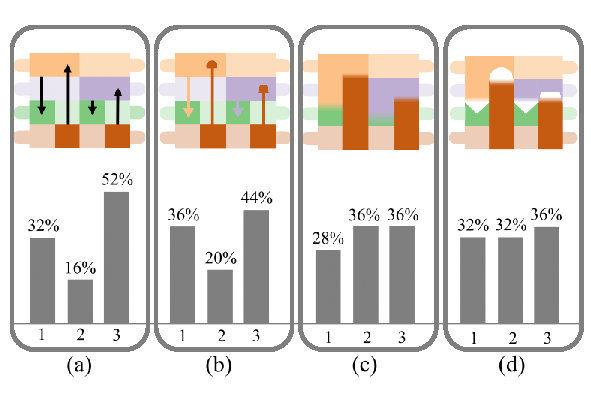
\includegraphics[width=0.48\textwidth]{Fig/statistic2.pdf}
	\vspace{-2em}
	\caption{Design scheme statistics.The statistical results of each group of design schemes are visual mapped with a histogram. The design with the highest selection is placed on top.}
	\vspace{-0.5em}
	\label{fig:sta}
\end{figure}

%我们对统计结果进行了分析。从图10中可以看到在四类设计案例中没有像素图边框的设计都是最受欢迎的。这种现象可以用格式塔理论进行解释。格式塔是一种心理学运动,其重要的观点是:人们对客观现象的感受源于整体关系而非具体元素。整体先于元素,局部元素的性质是由整体的结构关系决定的。这是因为人类对于任何视觉图像的认知是经过知觉系统组织后的形态与轮廓。格式塔理论可以应用到视觉组件的设计原则中。其原则包括:简单性,图形与背景关系,接近性,相似性,共向性,对称性,平行性,连续性,封闭性,共同区域,元素连通性。
After analyzing the statistical results against the design schemes, we find that the design without pixel map borders is the most popular in all four categories of design schemes as seen in Fig~\ref{fig:sta}. \textbf{Gestalt}~\cite{koffka_principles_2013, behrens_art_1998} theory can be used to explain this phenomenon. Gestalt is a psychological movement in which the important idea is that people's perceptions of objective phenomena originate from overall relationships rather than specific elements. The whole precedes the elements, and the nature of local elements is determined by the structural relationships of the whole. This is because human perception of any visual image is organized by the perceptual system in terms of form and contour. Gestalt theory can be applied to the design principles of visual components, including proximity, similarity, continuity, closure, common fate, good figure, symmetry, past experience. From the conclusions in Tab~\ref{tab:jf} and Tab~\ref{tab:es}, we choose Fig~\ref{fig:DC}.(d).3 as the legend for the display.

%表格2绘制
\renewcommand{\arraystretch}{1.3}
\newcolumntype{Y}{>{\centering\arraybackslash}X}
\begin{table}[h]
	\centering
	\caption{Matching Gestalt Theory}
	\begin{tabularx}{0.48\textwidth}{| c | Y | Y | Y | Y |}
		\hline
		\diagbox{Gestalt Theory}{Scheme} & (a).3 & (b).3 & (c).3 & (d).3  \\
		\hline
		Good figure     & \checkmark & \checkmark & \checkmark & \checkmark     \\
		\hline
		Continuity      & \checkmark & \checkmark & \checkmark & \checkmark     \\
		\hline
		Similarity             &  & \checkmark & \checkmark & \checkmark     \\
		\hline
		Closure                &  &  & \checkmark & \checkmark     \\
		\hline
		Proximity          &  &  & \checkmark & \checkmark     \\
		\hline
		{\makecell{Common fate}}        &  &  &  &      \\
		\hline
		Symmetry               &  &  &  &      \\
		\hline
		Past experience               &  &  &  &      \\
		\hline
	\end{tabularx}
    \label{tab:es}
    \vspace{0em}
\end{table}



%     6    %   案例分析
\section{EVALUATION}
%在这一章节,我们做了几个案例,选取了两个文本数据的案例来评估¥E^2$Storyline的可用性和有效性。第一个数据是电影\textit{纳尼亚传奇:狮子、女巫和魔衣橱}的文字概要。我们从维基百科中获取了电影的文字简介,并借助电影本身作为辅助。 第二个数据是 2015-2016 年 \textit{the Champions League} Round 16 第一回合的实时文字评论,当时阿森纳主场迎战巴塞罗那。我们使用$E^2$Storyline描述上述数据中的实体、实体关系及重要事件。
\noindent In this section, we make several case studies and select two cases of text data to evaluate the usability and effectiveness of $E^2$Storyline. The first data is the textual synopsis of movie \textit{The Chronicles of Narnia: The Lion, the Witch and the Wardrobe}. We obtained a text synopsis of it from Wikipedia, aided by the movie itself. The second data is a live text commentary about the first leg of \textit{the Champions League} Round 16 in 2015-2016, when Arsenal hosted Barcelona. The usefulness and scalability of $E^2$Storyline is further illustrated by a case study of this match data. We use $E^2$Storyline to describe the entities, entity relationships and significant events in the above data.

%   6.1   电影简介
\subsection{Text synopsis of a movie}
%图11,展示了电影\textit{The Chronicles of Narnia: The Lion, the Witch and the Wardrobe}的故事演变。可以看出,故事由几个主要的事件组成。参与同一事件的实体被很好的聚集在了一起。我们将实体间的关系分为三类,中立,友善和恶意,分别用梯形、半圆形和三角形表示。
Fig~\ref{fig:first} illustrates the story evolution of the movie \textit{The Chronicles of Narnia: The Lion, the Witch and the Wardrobe}. It can be seen that the story consists of several main events. The entities involved in the same event are well brought together. We classify relationships between entities into three categories, neutral, friendly and malicious, represented by ``\raisebox{-1mm}{
\includegraphics[scale=0.015]{Fig/mixcbg4.png}} ", `` \raisebox{-1mm}{
\includegraphics[scale=0.15]{Fig/mixcbg2.png}} ", `` \raisebox{-1mm}{
\includegraphics[scale=0.15]{Fig/mixcbg3.png}} ", respectively. 

%我们基于该数据,通过一个用户任务来验证$E^2Storyline$的直观性和有效性。我们参考了Brehmer等人的工作设计了以下9个任务。任务1到4属于基于事件的,任务5到8属于基于实体的,另外还有一个基于主观的任务9。对每个任务的答案,我们给出了一个基准。任务分类和基准如下表所示。
Based on this movie data, we evaluated the intuitiveness and effectiveness of $E^2$Storyline through a user study.
We took the task framework of Brehmer et al.'s multi-level typology~\cite{brehmer_multi_2013} into consideration and designed the following 9 tasks.
Tasks 1 to 4 are designed based on events, Tasks 5 to 8 are designed based on entities, and Task 9 is based on subjective design.
For the answer to each task, we give a ground truth. The task details are shown in the table in Fig.~\ref{fig:usertask}.
User tasks are as follows:
\begin{figure}[h]
	\centering
	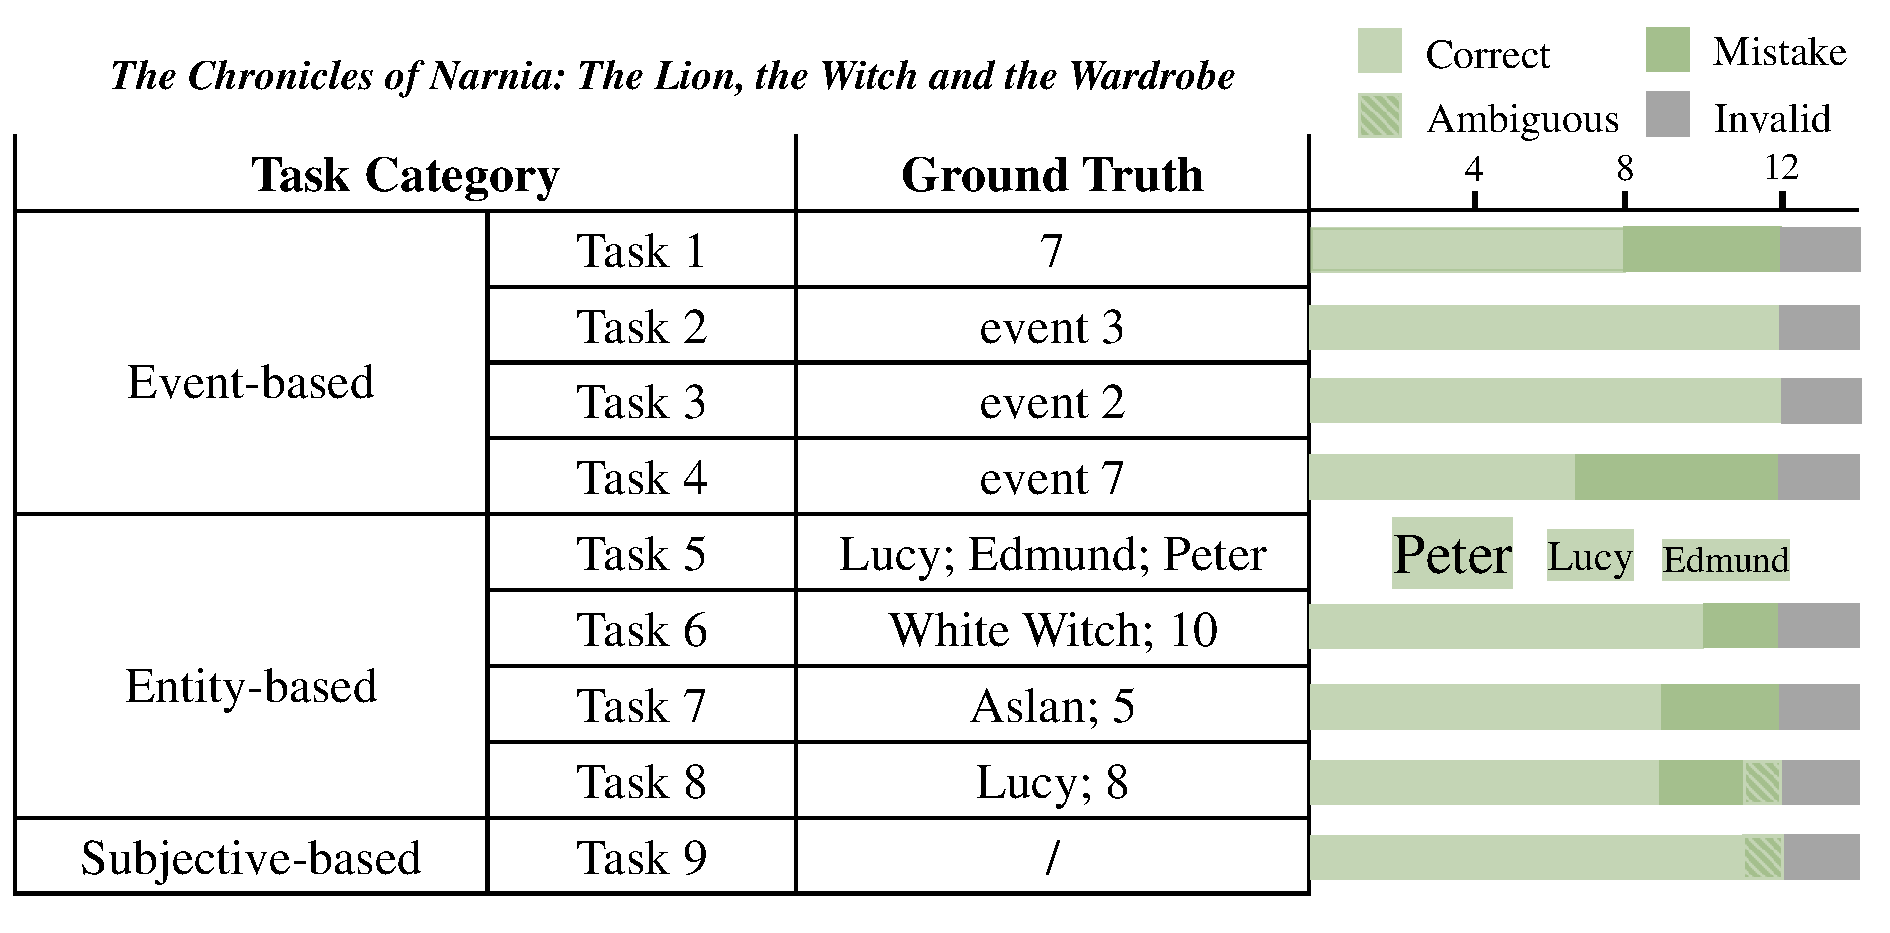
\includegraphics[width=0.48\textwidth]{Fig/usertask_stas.pdf}
	\vspace{-0.5em}
	\caption{9 user tasks, ground truth, and statistical results based on the user study.}
	\vspace{-0.5em}
	\label{fig:usertask}
\end{figure}

\textbf{Task 1:} Please answer the number of events included in the storyline.

\textbf{Task 2:} Please indicate the event with most participating entities.

\textbf{Task 3:} Please indicate the event with least participating entities.

\textbf{Task 4:} Please indicate the event with most complex entity relationship.

\textbf{Task 5:} Please choose the 3 most active characters in the whole story.

\textbf{Task 6:} Please select the most aggressive character and count the number of attack acts.

\textbf{Task 7:} Please select the friendliest character and count the number of acts of kind acts.

\textbf{Task 8:} Please select the most neutral character and count the number of neutral acts.

\textbf{Task 9:} Please analyze whether there is a group of entities acting in concert.

%%  电影 nania
%\begin{figure*}[t]
%	\centering
%	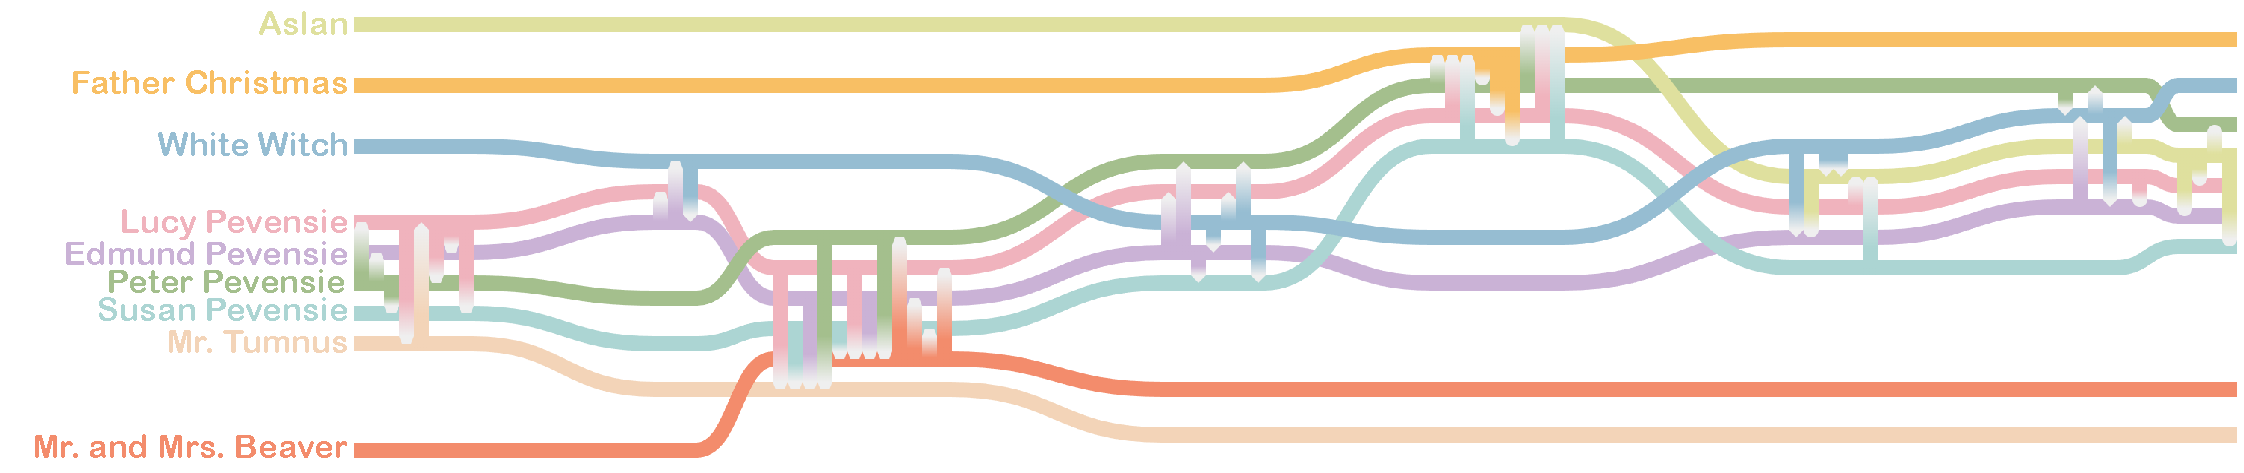
\includegraphics[width=\textwidth]{Fig/nania.pdf}
%	\caption{ \textit{The Chronicles of Narnia: The Lion, the Witch and the Wardrobe.} }
%	\label{fig:nania}
%\end{figure*}



%    表格3
%\renewcommand{\arraystretch}{1.5}
%\newcolumntype{Y}{>{\centering\arraybackslash}X}
%\begin{table}[h]
%	\caption{Task classification and corresponding benchmarks}
%	\centering
%	\begin{tabularx}{0.4\textwidth}{| c | c | Y|}
%		\hline
%		\multicolumn{2}{|c|}{Task Category} & {Benchmark}  \\
%		\hline
%		\multirow{4}{*}{Event-based} {\centering}
%		& Task 1    & 8                        \\
%		\cline{2-3}
%		& Task 2    & event 3                        \\
%		\cline{2-3}
%		& Task 3    & event 2                       \\
%		\cline{2-3}
%		& Task 4    & event 7                      \\
%		\hline
%		\multirow{4}{*}{Entity-based} {\centering}
%		& Task 5    & Lucy; Edmund; Peter                        \\
%		\cline{2-3}
%		& Task 6    & White Witch; 10                       \\
%		\cline{2-3}
%		& Task 7    & Aslan; 5  					\\
%		\cline{2-3}
%		& Task 8    & Lucy; 8                       \\
%		\hline
%		\makecell{Subjective-based}
%		& Task 9    &  /                      \\
%		\hline
%	\end{tabularx}
%	\label{tab:task}
%\end{table}

%我们邀请了14名参与者完成上述任务。他们中有2名为本科生,8名为研究生,2名博士生。XXX名有数据分析的经验,XXX名一直关注可视化领域的研究。统计结果如下图所示。
%我们通过邮件在智能感知研究所招募了xx名参与者(xx名男性和xx名女性,年龄在xxx之间)。
We recruited fourteen participants (eight males and six females, aging from 20-27) through an students email list.
%xx名参与者是本科生,xx名参与者是研究生。
Three participants were undergraduate students and eleven participants were postgraduate.
%xx人有数据分析方面的实践经历,xx人从事计算机视觉的相关研究,xx人熟悉数据可视化...
Six had practical experience in data analysis, three were engaged in computer vision related research, three were understand data visualization.
%其他xx名的技术背景有限,但对可视分析有着浓厚的兴趣,且学习过数据可视化、网页设计、人机交互等课程。
The other two had limited technical backgrounds but had a strong interest in visual analysis, and had studied data visualization, web design, human-computer interaction and other courses.
%除了了解参与者的个人信息,我们还确保所有参与者没有色盲或色弱方面的视觉认知障碍,在理解视觉映射方面没有困难。
In addition to knowing the personal information of the participants, we also ensured that all participants had no visual cognitive impairment in terms of color blindness or color weakness, and had no difficulty in understanding visual mapping.
%我们使用了一台笔记本电脑,xx英寸显示屏,分辨率为xxxxx像素。
A laptop computer was used, with a 25-inch display of resolution 1920$\times$1080 pixels.

%首先,我们花费平均5-8min向参与者介绍MDEStoryline,数据背景,和用户任务。
First, each participant started with an around 5 minute tutorial, introducing the $E^2$Storyline, data context, and user tasks.
%其次,我们确保每位参与者独立完成用户任务。在参与者执行任务期间,只允许一名评估主持者和一名评估记录者在场,且不允许这两位工作人员干预参与者的任务执行。
Second, we ensured that each participant completes user tasks independently. Only one assessment facilitator and one assessment recorder were allowed to be present during the participants's task performance, and the two staff were not allowed to interfere with the participant's task performance.
%然后,我们要求参与者依次执行用户任务,给出个人见解。此外,待用户任务执行完毕后,调研主持者以访谈的形式与参与者进行交流,了解参与者的主观反馈。
Then, we asked the participant to perform user tasks and give personal insights based on evaluation indicators.
%用户任务的执行过程以及访谈内容均由调研记录者进行实时记录。
The execution process of user tasks and the interview content are recorded in real time by the assessment recorder.

%我们整理每个用户任务的反馈结果,统计了回答正确,错误和不清楚的人数,统计结果呈现在图11的堆栈图中。在14位参与者中,有2位曾经看过本部电影,因此我们将这2个反馈作为无效样本。
We collated the feedback results for each user task, and counted the number of people who answered correctly, mistake, and ambiguous. The statistical results are presented in the stack diagram in Fig~\ref{fig:usertask}. Two participants had prior knowledge of this work, so we took these two feedback results as invalid samples.

%在基于事件的用户任务中,我们发现参与者在分析过程中比较关注事件的聚集区域,而忽视实体本身的信息。例如在任务1中,4位参与者认为该故事线呈现了7个事件,他们忽视实体Susan Pevensie的故事线并没有在空间上向事件7逼近,因为误认为事件7和事件8属于同一个事件。另外,7位参与者认为最复杂的事件是事件3,他们只关注到该事件参与的实体数量较多,事件所占像素空间较大,但是他们忽视了实体之间的行为。事件7中涉及的实体关系和行为类型相较于事件3更为杂乱。
In the event-based user tasks, we found that the participants paid more attention to the gathering area of the event during the analysis process, while ignoring the information of the entity itself. For example, in Task 1, 4 participants hold that the story contained 7 events. They ignored the storyline of entity Susan Pevensie, which doesn't approach
to event 7 in space, but to event 8. So they mistakenly thought that event 7 and event 8 belong to the same event. In addition, 7 participants hold that the most complex event was event 3. They only focused on the large number of entities involved in the event, and the event took up a large pixel space, but they ignored the behavior between entities.

%在基于实体的用户任务中,我们发现大部分参与者能够基于$E^2Storyline的视觉设计,通过分析实体之间的关系和行为类型,来区分故事中的实体,了解他们的角色定位。少部分参与者不够熟悉我们的行为类型设计方案,导致他们的分析结果出现错误,尤其在统计行为数目上。极少的参与者不能清晰的分辨。
In the entity-based user tasks, we found that most of the participants were able to distinguish the entities in the story and understand their role positioning by analyzing the relationship and behavior types between entities based on the visual design of $E^2$Storyline. Few participants were not familiar enough with our behavioral type design scheme, leading to errors in their analysis, especially in counting the number of behaviors. Few participants were ambiguous about the results.

%在基于主观的用户任务中,我们要求参与者探索故事中是否存在实体帮派。其中,10位参与者都讲出来他们认为的实体帮派,如故事3中,Lucy、Edmund、Peter三人是一个团体,他们3人向Mr.Tumnus和Mr. and Mrs. Beaver施加中立行为。如图1.(A1)所示。如故事5中,圣诞老人对他们3人施加友善行为。如图1.(A2)所示。
In a subjective-based user tasks, we asked participants to explore the presence of entity group in the story.
Ten participants hold that they had discovered the entity group.
For example, as shown in Fig~\ref{fig:first}.(A1) and Fig~\ref{fig:first}.(A2), ``Lucy Pevensie, Edmund Pevensie, and Peter Pevensie were a group, and they imposed neutral behavior on Mr.Tumnus and Mr. and Mrs. Beaver."  ``Father Christmas imposed friendly behavior on them."

%除此之外,我们还询问参与者关于故事线的可解释性和可用性的反馈。约71.5%的参与者认为我们的故事线理解起来比较容易,约85%的参与者认为我们的故事线能够帮助理解故事、事件及实体关系。还有3位参与者主动询问我们事件4是否为整个故事的转折事件,因为该事件中的关系类型多为恶意的,这与之前的都不一样。这说明$E^2$Storyline可以帮助用户发现事件的在整个故事中的功能。
Morover, we collated participant feedback on the interpretability and usability of $E^2$Storyline. About 71.5\% of the participants hold that $E^2$Storyline were easy to understand, and about 85\% of the participants believed that $E^2$Storyline helped to understand story, event, and entity relationships. Three participants volunteered to ask us whether event 4 was a turning event in the story, because they found that the type of relationship between entities in event 4 was mostly malicious, which is different from all previous ones. It shows that $E^2$Storyline can help users discover the function of events in the whole story.

%我们还对电影红番区和黑客帝国做了展示,然后询问参与者观察这两部电影的故事线可视化直观感受。图12展示了电影红番区的故事演变。数量较多的参与者认为该故事中类型为恶意的关系数量最多,认为这部电影可能是动作片。事实上,红番区的电影类型确实是动作片。这说明$E^2$Storyline可以在一定程度上帮助用户判断电影的类型。图13展示了电影黑客帝国的故事线可视化。有部分参与者认为,电影中的角色“墨菲斯”是好人,因为涉及他的关系类型大多数都是善意的。事实上,墨菲斯在电影中的角色的确是个好人。这说明$E^2$Storyline可以帮助用户判断实体的身份。
We also made a presentation of the movies \textit{Rumble in the Bronx} and \textit{The Matrix}, and then asked the participants how they intuitively felt after observing the story line visualizations of the two films. Fig~\ref{fig:hfq} illustrates the story evolution of the movie \textit{Rumble in the Bronx}. The larger proportion of participants observed that ``malicious" relationships were the most frequent of the three genres. Therefore they believed that the movie was an action movie with a high probability. In fact, the film's genre is indeed action. This shows that $E^2$Storyline can help users to determine the movie genre to some extent. Fig~\ref{fig:matrix} shows a storyline visualization of the movie \textit{The Matrix}. Some participants believed that the character ``Morpheus" in the movie was a good guy because most of the types of relationships involving him were friendly. Actually, Morpheus is indeed a good guy in the movie. This suggests that $E^2$Storyline can help users determine the identity of entities.

%   6.2   足球直播数据
\subsection{Live text streaming of a football game}
%在没有原始视频上下文的情况下,实时文本评论用于描述即时比赛或新闻的实时报道。实时文本数据主要用于在线直播体育比赛,也用于实时报道各种其他新闻事实。为了满足即时性,实时文本数据中的句子具有简短的特点,但也保留了句子的一般结构。 因此,我们可以从数据中提取结构化的三元组信息。此外,实时文本几乎没有时间跳跃,因此在时间上具有高度线性的特点。
In the absence of raw video context, live text commentary is used to describe live reports of instant matches or news. Live text data is mainly used for live online streaming of sports matches, but also for live coverage of various other news facts. To meet the immediacy of reporting, the sentences in live text data are characterized by shortness, but also preserve the general structure of sentences. Therefore, we can extract structured SPO triples from the data. Moreover, there are almost no time jumps in live text commentary, so it is highly linear in time.

%赛后集锦被作为选择事件的依据,我们用$E^2$Storyline从2个角度对这场足球比赛进行可视化。1.阿森纳的中场和前场球员对阵巴塞罗那的中场和后场球员,2.巴塞罗那的中场和前场球员对阵阿森纳的中场和后场球员。我们用半圆表示进攻,梯形表示防守,三角形表示进球,灰色的虚线表示中场休息。我们从这两个视角分别得到了一些结论,这让我们更全面的了解这场比赛。
The post-match highlights were used as the basis for selecting the event, and the soccer match was visualized from 2 perspectives using $E^2$Storyline. The two perspectives are: \ding{182} Arsenal’s midfield and front players against Barcelona’s midfiel and back players, as shown in Fig~\ref{fig:fba2b}.  \ding{183} Barcelona’s midfield and front players against Arsenal’s midfield and back players, as shown in Fig~\ref{fig:fbb2a}. We use `` \raisebox{0mm}{
\includegraphics[scale=0.15]{Fig/mixcbg3.png}} " for offense, ``\raisebox{0mm}{
\includegraphics[scale=0.015]{Fig/mixcbg4.png}} " for defense, `` \raisebox{0mm}{
\includegraphics[scale=0.15]{Fig/mixcbg2.png}} " for goals, and gray dotted lines for halftime. We got some conclusions from each of these two perspectives, which gives us a more comprehensive understanding of the game.

%  足球图
\begin{figure*}[t]
	\centering
	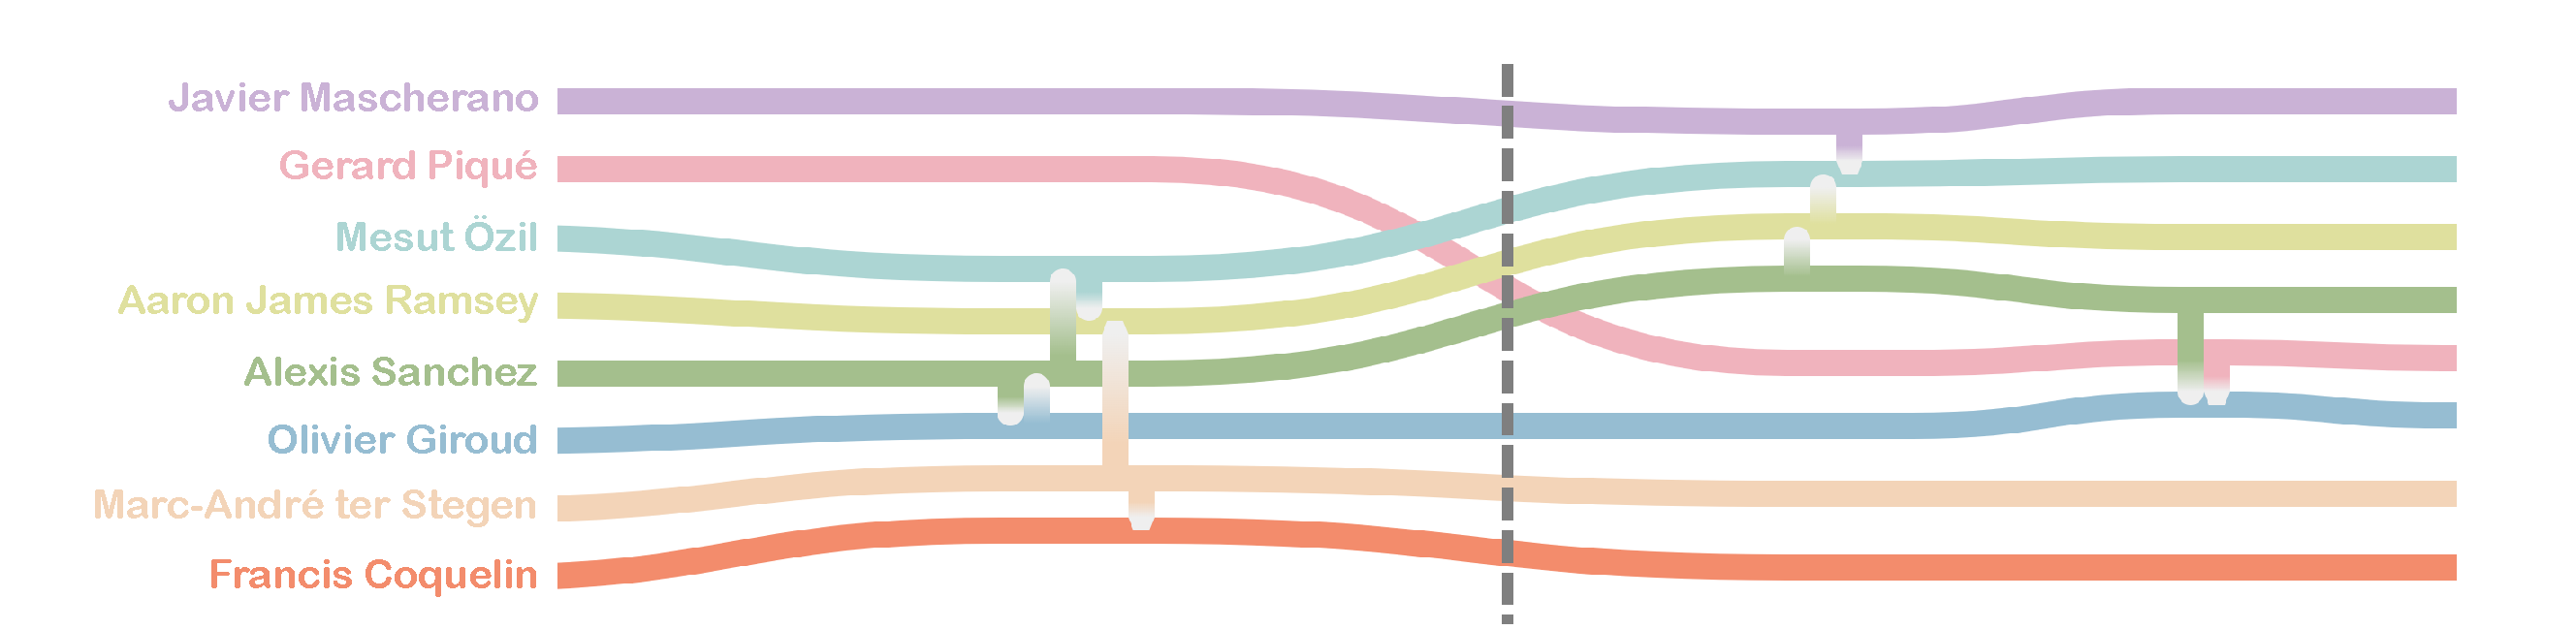
\includegraphics[width=\textwidth]{Fig/A2B.pdf}
		\vspace{-1.5em}
	\caption{ \textit{Arsenal’s midfield and front players against Barcelona’s midfiel and back players.} }
		\vspace{0em}
	\label{fig:fba2b}
\end{figure*}

\begin{figure*}[t]
	\centering
	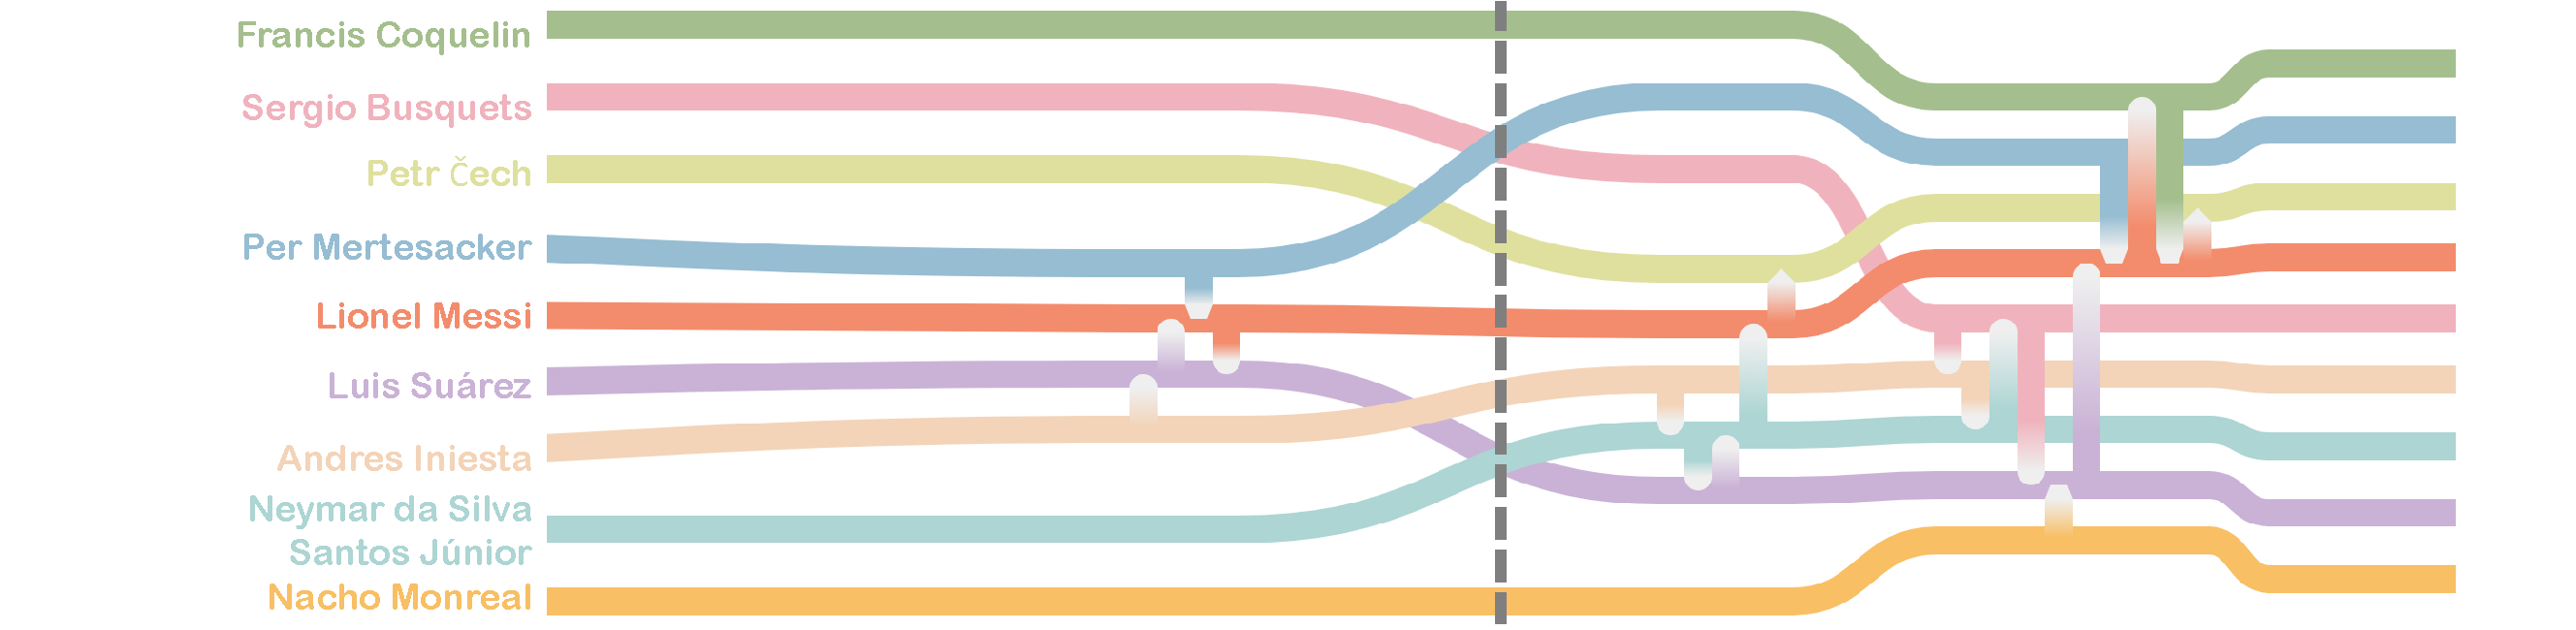
\includegraphics[width=\textwidth]{Fig/B2A.pdf}
		\vspace{-1em}
	\caption{ \textit{Barcelona’s midfield and front players against Arsenal’s midfield and back players.} }
		\vspace{-1em}
	\label{fig:fbb2a}
\end{figure*}


%图14为阿森纳前场球员进攻巴塞罗那的后场球员。可以从图14中看出,集锦视频中阿森纳最活跃的进攻发生在上半场。在阿森纳的进攻球员中桑德斯是最活跃的球员。我们对阿森纳的进攻不多的原因进行了探索,发现阿森纳的进攻球员和巴萨的防守球员数量相同。我们还可以发现,阿森纳的进攻多是有桑切斯(左边锋)发起,传球给吉鲁(中锋),巴塞罗那的防守球员是马斯切拉诺和皮克(中后卫),这说明阿森纳的战术多为正面进攻。这符合阿森纳“4-2-3-1”的阵型。
\textbf{Perspective \ding{182}:} The following information can be obtained from Fig~\ref{fig:fba2b}. First, Arsenal's most active offense occurred in the first half. Second, Among Arsenal's attacking players Sanchez was the most active player. Most of Arsenal's attacks were initiated by Sanchez (left winger) and passed to Giroud (center forward), while Barcelona's defenders were Mascherano and Piqué (center backs), indicating that Arsenal's tactics were mostly frontal attacks. This is in line with Arsenal's ``4-2-3-1" formation. The figure also suggests that the reason for Arsenal's lack of offense may be Barcelona's good defense (Arsenal has the same number of offensive players as Barcelona's defensive players).


%图15为巴塞罗那前场球员进攻阿森纳的后场球员。从图15中看出巴塞罗那在下半场活跃。巴塞罗那的两个进球都是梅西。巴萨的球员之间互动较多,尤其是苏亚雷斯、内马尔和梅西之间。巴萨的进攻球员数量比阿森纳的防守球员更多,其进攻更为顺畅。巴塞罗那的进攻球员数量比阿森纳的防守球员更多,其进攻更为顺畅。
\textbf{Perspective \ding{183}:} The following information can be obtained from Fig~\ref{fig:fbb2a}. First, Barcelona was more active in the second half than in the first half. Second, Barcelona's players had more interaction with each other, especially Suarez, Neymar and Messi. The two attacks that led to the goal were both launched from Barcelona's left side. Neymar and Suarez drew the Arsenal defenders and finally passed the ball to Messi to shoot and score.


%     7    %   讨论和未来工作
\section{DISCUSSION {\&} FUTURE WORK}
%在本节,我们回顾了整个工作流程,基于案例和用户反馈,全面讨论$E^2Storyline$的优点和限制,并思考未来的工作。
\noindent In this section, we review the entire workflow, discuss the advantages and limitations of $E^2$Storyline in a comprehensive manner based on case studies and user feedback, and reflect on future work.

%我们认为在故事线中仅仅反映故事发展趋势是不够的。事件中实体间的关系同样非常重要。为此我们提出了$E^2Storyline$,一个新的故事线布局。我们从文本数据中提取SPO三元组,用它来描述实体之间的关系。我们遵循公认的故事线的可视设计原则,还提出了一些自定义的设计需求。我们用多目标优化问题描述故事线布局优化,并使用Gurobi求解。针对实体间关系的可视表达,我们进行了头脑风暴,对不同的设计方案做了用户调研。我们用“电影文字简介“和“一个文本直播评论”做了案例分析。总的来说,我们发现参与者使用$E^2$Storyline可以快速准确的找到故事中的重要事件,并且能进一步分析出事件的作用和实体的一些模式。
We believe that it is not enough to reflect story trends in storyline visualization. The relationships between entities in events are equally important. To do this we propose $E^2$Storyline, a novel storyline layout. We extract SPO triples from texual data and use them to describe the relationships between entities. We followed the accepted visual design principles for storyline and also came up with some custom design requirements. We described layout of storyline using a multi-objective optimization problem and solved it with \textit{Gurobi}. For the visual representation of the relationships between entities, we brainstormed and did user studies on different design schemes. We made case studies with movie text synopsis and live text commentaries. Overall, we found that participants using $E^2$Storyline could quickly and accurately find important events in the story and could further analyze the role of events and some patterns of entities.

%算法。布局优化需要将多个设计需求进行综合考虑,因此我们将其表述成多目标优化问题。它可以使用Gurobi求解得到全局最优,保证了该布局是最符合设计需求的。随着数据规模增大,受限于gurobi的效率,求解全局最优会花费更多的时间。这就使得算法的实时性不佳。在未来工作中,我们将尝试构建一些规则来精简数据规模。为了克服实时性差,在未来工作中,我们将进行一下几种尝试。1、构建一些规则来预处理数据,以减少规模。2、使用多种算法结合的方式,比如多目标优化+遗传算法。
\textbf{Algorithm.} Layout optimization requires the integration of multiple design requirements, so we formulate it as a multi-objective optimization problem. It can be solved using Gurobi to obtain the global optimum, which ensures that the layout is the best fit to the design requirements. As the size of the data increases, limited by the efficiency of gurobi, solving the global optimum will cost more time. This makes the algorithm poor in real time. To overcome the poor real-time performance, in future work, we will make several attempts. \ding{182} Construct some rules to pre-process the data to reduce the size. \ding{183} Multiple algorithms work together, such as multi-objective optimization + genetic algorithm. \ding{184} Use machine learning to solve layout optimization problems.

%可视设计。通过头脑风暴和用户研究,我们确定了一个视觉设计方案来显示实体之间的关系。这个视觉设计方案具有良好的指向性(颜色渐变),同时向用户传达了行动的类型(基础图形),没有增加复杂性。从案例研究中可以看出,这种设计方案是有效的。然而,由于基础图形的多样性,这种设计方案不能表达太多的行动类型。为了对表达更多关系,下一步,我们将会探索其他的可视设计方案,以及增加例如高亮,框选等交互功能。
\textbf{Visual design.} Through brainstorming and user studies, we identified a visual design scheme to show the relationships between entities. This visual design scheme has good directionality (color gradients) while conveying the type of action (base graphics) to users without adding complexity. It is clear from the case studies that this design scheme is effective. However, this design scheme cannot express too many types of relations due to the variety of base graphics. In order to express more relationships, we will next explore other visual design schemes and add interactive features such as highlighting and boxing.

%总的来说,故事线可视化作为概览故事趋势的手段是快速的且有效的。未来在故事线可视化的图例设计,以及提出更高效的布局算法方面仍有研究价值。
Overall, storyline visualization is useful and effective as a method of providing an overview of story trends. There remains value for future research in the design of legends for storyline visualization and in proposing more efficient layout algorithms.


%     8    %   结论
\section{CONCLUSION}
%我们提出了一种新的故事线布局方法,着重于展示组成故事的各个事件中实体之间的关系。我们对数据和可视设计两者进行了针对性的需求分析,综合这些需求将故事线布局准换成多目标优化问题。我们列举了多个案例,并进行用户调研。结果表明,我们的参与者在使用$E^2$Storyline时,可以较快的找到故事中的事件。同时,参与者对事件的作用,实体之间的关系也能展开快速有效的分析。
\noindent We proposed a novel method of storyline layout that focuses on showing the relationships between entities in the various events of the story. We performed a tailor-made requirements analysis for both data and visual design, and described the storyline layout with a multi-objective optimization problem mathematically. We cite several case studies and conduct user studies. The results show that our participants can quickly find the events in the story when using $E^2$Storyline. Participants were also able to develop an efficient and effective analysis of the roles of events, and relationships between entities.



%% if specified like this the section will be committed in review mode
\acknowledgments{
The work is partly supported by the National Key Research and Development Program of China (2020YFB1707700), National Natural Science Foundation of China (61972356, 62036009), Fundamental Research Funds for the Provincial Universities of Zhejiang (RF-A2020001).}

%\bibliographystyle{abbrv}
\bibliographystyle{abbrv-doi}
%\bibliographystyle{abbrv-doi-narrow}
%\bibliographystyle{abbrv-doi-hyperref}
%\bibliographystyle{abbrv-doi-hyperref-narrow}

\bibliography{template}
\end{document}
